\documentclass{estiloDeTesis}
\usepackage[sort]{natbib}
%\renewcommand{\bibAnnoteFile}[1]{%
%\IfFileExists{#1}{\begin{quotation}\noindent\texts c{Key:} #1\\
%\textsc{Annotation:}\ \input{#1}\end{quotation}}{}}
%\renewcommand{\bibAnnote}[2]{%
%\begin{quotation}\noindent\textsc{Key:} #1\\
%\textsc{Annotation:}\ #2\end{quotation}}
\usepackage[T1]{fontenc}
\usepackage{mathrsfs}
\usepackage{makeidx}
\usepackage[breaklinks=true]{hyperref}
\usepackage{breakcites}
\hypersetup{breaklinks=true,colorlinks=true,linkcolor=black,citecolor=black,urlcolor=black}
\usepackage{algorithm}
\usepackage{algorithmic}
%\floatname{algorithm}{Algoritmo}
\renewcommand{\listalgorithmname}{Lista de algoritmos}
\renewcommand{\algorithmicrequire}{\textbf{Entrada:}}
\renewcommand{\algorithmicensure}{\textbf{Salida:}}
\renewcommand{\algorithmicend}{\textbf{}}
\renewcommand{\algorithmicif}{\textbf{Si}}
\renewcommand{\algorithmicthen}{\textbf{Entonces}}
\renewcommand{\algorithmicelse}{\textbf{Else}}
\renewcommand{\algorithmicelsif}{\algorithmicelse,\ \algorithmicif}
\renewcommand{\algorithmicendif}{\textbf{Fin}\ \algorithmicif}
\renewcommand{\algorithmicfor}{\textbf{Para}}
\renewcommand{\algorithmicforall}{\textbf{For All}}
\renewcommand{\algorithmicdo}{\textbf{Hacer}}
\renewcommand{\algorithmicendfor}{\textbf{Fin}\ \algorithmicfor}
\renewcommand{\algorithmicwhile}{\textbf{Mientras}}
\renewcommand{\algorithmicendwhile}{\textbf{Fin}\ \algorithmicwhile}
\renewcommand{\algorithmicloop}{\textbf{Loop}}
\renewcommand{\algorithmicendloop}{\textbf{Fin}\ \algorithmicloop}
\renewcommand{\algorithmicrepeat}{\textbf{Repeat}}
\renewcommand{\algorithmicuntil}{\textbf{Until}}
\renewcommand{\algorithmicprint}{\textbf{Print}} 
\renewcommand{\algorithmicreturn}{\textbf{Retornar}} 
\renewcommand{\algorithmictrue}{\textbf{Verdadero }} 
\renewcommand{\algorithmicfalse}{\textbf{Falso }} 

\usepackage{pstricks}
\usepackage{url}
\usepackage{doi}
\usepackage{lscape}
\usepackage{color}
\usepackage[pdftex]{graphicx}
%\usepackage{graphicx}
\usepackage{epstopdf}
\usepackage{epsfig}
\usepackage{footnote}
\usepackage{longtable}
\usepackage{array}
\usepackage[section]{placeins}
\usepackage[margin=10pt,font=small,labelfont=bf,labelsep=endash]{caption}
\usepackage{subcaption}
\usepackage{listings}
\def\titulo{{Applying Homomorphic Encryption in the Cloud}}
\def\autor{Jes\'{u}s Antonio Soto Vel\'{a}zquez}
\def\grado{Ingeniero en Tecnolog\'{i}a de Software}
\def\matricula{1570031}
\def\fecha{14 de julio de 2015}
\def\asesor{Dra.\ Sara Elena Garza Villarreal}
\def\coasesor{Dra.\ Elisa Schaeffer}
\def\revisor{Dr.\ Sergio Fernando Alcaraz Corona}
\def\vobo{Dr.\ Arnulfo Trevi\~{n}o Cubero}
\newcommand{\pname}[1]{{\fontfamily{phv}\selectfont{#1}\fontfamily{cmr}\selectfont}}
\renewcommand{\lstlistingname}{Code Snippet} 
\renewcommand{\lstlistlistingname}{List of \lstlistingname s}
\setcounter{secnumdepth}{5}
\makeindex

%Paquete para texto de color
\usepackage{color}
\definecolor{red}{rgb}{1.0,0,0}
\definecolor{blue}{rgb}{0,0,1.0}
\newcommand{\comentario}[1]{\textcolor{red}{\textbf{#1}}} %Comentarios asesor
\newcommand{\correccion}[1]{\textcolor{black}{\text{#1}}} %Correcciones alumno
\newcommand{\captionFigureCorrection}{\vspace*{-6mm}}
\newcommand{\captionSubfigureCorrection}{\vspace*{-5mm}}
%\renewcommand{\tablename}{Cuadro}
%\usepackage{ulem}
\usepackage{hhline}

\makeglossary
\makeindex

\begin{document}

\frontmatter
\pagestyle{main}
\def\uanl{Universidad Aut\'{o}noma de Nuevo Le\'{o}n}
\def\fime{Facultad de Ingenier\'{\i}a Mec\'{a}nica y El\'{e}ctrica}
\def\depg{Divisi\'{o}n de Estudios de Licenciatura}
\def\snnl{San Nicol\'{a}s de los Garza, Nuevo Le�n}
\thispagestyle{empty}

\begin{scshape}
\begin{center}
	{\Large \uanl} \\[6mm]
	{\large \fime} \\[6mm]
	{\large \depg}
	\vskip 16mm
	
\includegraphics[height=55mm]{uanl}
	\vskip 14mm
%	\begin{tabular}{p{11cm}
%        \begin{tabular}{p{11cm}}       
         \centering              {\large \titulo}
%	\end{tabular}
	\vskip 8mm
	{por}\\[8mm]
	{\large \autor}\\[8mm]
	{en opci\'{o}n al grado de}\\[3mm]
	{\large \grado}\\
\end{center}

\vfill
\snnl \hfill \fecha
\end{scshape}

\newpage
\thispagestyle{empty}

\begin{scshape}
\begin{center}
	{\Large \uanl} \\[6mm]
	{\large \fime} \\[6mm]
	{\large \depg}
	\vskip 17mm
	
\includegraphics[height=50mm]{fime}
	\vskip 17mm
%	\begin{tabular}{p{11cm}}
		\centering		{\large \titulo}
%	\end{tabular}
	\vskip 8mm
	{por}\\[8mm]
	{\large \autor}\\[8mm]
	{en opci\'{o}n al grado de}\\[3mm]
	{\large Ingeniero en Tecnolog\'{i}as de Software}
\end{center}

\vfill
\snnl \hfill \fecha
\end{scshape}

\newpage
\thispagestyle{empty}
\enlargethispage{5mm}

\begin{center}
{\bf \large \uanl} \\
{\bf \fime} \\
{\bf \depg}
\end{center}
\vskip 5mm

Los miembros del Comit\'{e} de Tesis recomendamos que la
Tesis \guillemotleft \titulo \guillemotright, realizada
por el alumno \autor, con n\'{u}mero de matr�cula \matricula, sea
aceptada para su defensa como opci\'{o}n al grado de \grado.
\vskip 8mm

\begin{center}
El Comit\'{e} de Tesis\\          
\vskip 17mm

\begin{center}
\rule{70mm}{0.3pt}      

\vspace*{-3mm}

\asesor
\vspace*{-4mm}

Asesor
\end{center}

\vspace*{8mm}

\begin{tabular}{cc}
\rule{60mm}{0.3pt} & \rule{80mm}{0.3pt} \\
	\coasesor & \revisor \\
	Revisor & Revisor   \\
\end{tabular}

\vspace*{8mm}

\begin{center}
Vo.\ Bo.\

\vspace*{6mm}

\rule{60mm}{0.3pt}      

\vspace*{-6mm}

\vobo

\vspace*{-3mm}

\depg
\end{center}

\vfill

\snnl, \fecha

\end{center}

\chapter*{Acknowledgements}

I would like to thank all the people who made this dissertation possible, starting with my wonderful professors in the Faculty of Mechanic and Electrical Engineering at Autonomous University of Nuevo Le\'{o}n. 

Dr. Sara Elena Garza, who was both my committee chair and my first programming professor, has been of great influence towards my education on software engineering. From start to finish, she has shown great patience and never once gave up on me. She has always been a great source of motivation, helping me pull through both the classes I have taken under her, and also the projects I have collaborated with her. Whenever I strayed from my goals, her encouragement and positive attitude helped me get back in track. 

Dr. Elisa Schaeffer has always provided me with sound advice and inspiration, despite not having taking classes under her officially. The conversations I have held with her showed her passion towards the topics she teaches, which prompted me to become more engaged with other topics I was not familiar with. Dr. Sergio Alcaraz has been an invaluable professor for my education, and I greatly appreciate his patience and seriousness towards all the questions I asked during class. I had never before met a professor who seemed as pleased as he did whenever I asked questions, which motivated me to learn more of the subject and become engaged in his lectures. Dr. Iris Mart\'{i}nez and Dr. Preethy Rajesh are both amazing professors who have demonstrated that high quality education and kindness are not mutually exclusive. Finally, I would like to thank my professors from my student exchange at University of Ottawa during autumn 2012. Dr. Carlisle Adams introduced me to the world of cryptography, and because of his passion towards the subject, I became truly interested in learning about it, in spite of how complex it seemed.

My friends from Monterrey and Obreg\'{o}n city have provided me with the moral support I needed when I was writing my dissertation. I truly appreciate their kind words when I needed them the most, and also the brief distractions that helped me regain my perspective. In particular, I would like to thank Cassandra Delgado, Leticia Neaves, Alexis Rodr\'{i}guez, Luis Cano, Alan Ch\'{a}vez, Eduardo Villalobos, \'{E}rika Tapia, Marian Ju\'{a}rez, and Emilie Angel.

Finally, I would like to thank my family for their inconditional support, even as we are apart. Particularly, to my mother and role model Celia Vel\'{a}zquez, who throughout my life has supported me in all of my life goals and projects. 

\newpage

\chapter{Abstract}
\markboth{Resumen}{}

\noindent\autor.

\noindent Candidato para el grado de [Ingeniero en Tecnolog\'{\i}as de Software].
%\indent 

\noindent\uanl.\\
\noindent\fime.

\noindent T\'{\i}tulo del estudio: 

\begin{center}
\begin{tabular}{p{11cm}}
	\centering
	\scshape{\large{\titulo}}
\end{tabular}
\end{center}\bigskip

\noindent N\'{u}mero de p\'{a}ginas: \pageref*{lastpage}.

\paragraph{Objetives and Study Method}
%Problem
This work proposes an implementation of a client-server architecture based software that uses HElib to enable homomorphic encryption and perform computations on the encrypted data. Cloud computing is a cost-efficient alternative to host data remotely and subsequently perform computations on it. Confidentiality becomes an issue when data is delegated to the cloud, as often the information hosted is considered to be sensitive. A typical approach is to make use of a cryptographic algorithm that encrypts the data with a secret key that only the owner has. However, as long as the owner of the data wishes to make changes to the encrypted data, he would have to download the encrypted data, decrypt it using his secret key, perform the desired computations or changes to it, and reencrypt it once again before uploading it to the server in the cloud. An alternative to this approach is to make use of \emph{homomorphic encryption}, and advanced technique in cryptography that enables computations on encrypted data without needing the secret key. 

%Motivation
Homomorphic encrypting is a well-sounding alternative over the typical approach of encrypting data every time it is send to the cloud; however, so far the schemes that make this possible have been thought of as being too slow and expensive, storage wise. A library that implements homomorphic encryption, HElib, is based off an homomorphic encryption scheme that seems very promising because of the optimizations and improvements over other past schemes. Using HELib, it would be possible to reevaluate the situation and show to what degree it would be feasible to make a solution based on homomorphic encryption.

%Lo que proponemos
The proposed solution consists in taking the functionalities provided by HElib, and build a client-server based software that aims to address the main scenarios found in the proposed case study. Even though the proposed implementation could in theory work for a number of examples, it is designed taking into account the case study; therefore, both are closely related.

%Caso de Estudio
Consider the scenario where a household has an expected pattern of activity, ie. empty during the day and non-empty at night, so that the householder seeks to ascertain the number of people inside at any point in time during the day. Assuming the householder has put in place certain sensors around the building so that it detects and counts who comes in and out, he would like to learn the value of the counter remotely. As the householder chooses to store the value in the cloud, he quickly realizes he does not want others to learn of this value, not even the cloud service itself, as to prevent potential burglars to break in when the household is empty. Additionally, he wishes that the counter gets updated at certain intervals, e.g. every 20 minutes. 

%Problematica al encriptar cada vez
The problem found in encryping and then uploading the data every time a change is made, is that the overhead costs might be too high to do this often. For one, bandwidth would be spent on each ocassion, and the time required for encryption and uploading might not be that short. 

\paragraph{Contributions and Conclusions}
%Diferencia de los demas trabajos
In contrast with other works, the proposed solution tackles on the problem by employing homomorphic encryption. It is a simple client-server architecture which could be expanded to adapt with other scenarios and requirements. The proof of concept provides the means to operate on the encrypted data, ie. performing additions on the counter value, without compromising confidentiality and wasting resources caused by the overhead costs of reencrypting data at every change.

%Experimentos

To show the feasibility of using HElib to do homomorphic encryption, experiments were designed by varying the value of a security parameter $k$. This value has a direct impact on the execution time of key generation, encryption, and decryption, as well as the size of the resulting public key. The findings show that even though key generation time is long, taking approximately between 9 and 13 seconds, and key size is large, being between 35MB and 165M, it is not considered to be an issue, as this step is done one time only. On the other hand, encryption, decryption, and addition times are amazingly fast, none of them exceding over 1 second. However, the ciphertext raises some doubts over the magnitude of its size: during development, it was found that on average, ciphertext size was 74MB; meanwhile, during experimentation, it was found that ciphertext size rose no higher than 45kB. To the best of our knowledge, there is yet no way to predict the size of the ciphertext by using HElib. Therefore, if it were found to keep the size of the ciphertext below 45kB, it would certainly be feasible to take this solution to the cloud; otherwise, it would not be possible if each ciphertext had a size that exceded several MB.

\noindent Firma del asesor: \rule{72mm}{0.3pt}

\vspace*{-4mm}

\noindent \phantom{Firma del asesor: m} \asesor


\tableofcontents
\listoffigures
\listoftables
\lstlistoflistings

%\pagestyle{nom}
%\renewcommand\nomname{\'{\I}ndice de cuadros}
%\makenomenclature
%\printnomenclature[1in]
\clearpage
\pagestyle{main}
\newpage
%\printglossary
\mainmatter
\pagestyle{fime}
%%Aqui van tus abreviaciones
\nomenclature{NN}{Neural Network}
\nomenclature{HMM}{Hidden Markov Model}
\nomenclature{RGB}{Red Green Blue}
\newpage



% AQUI
\chapter{Introduction}
\label{intro}

Communication has always been a basic human need, and the means to do it are especially linked to the available technology. Thanks to the advances in techonology, it has become more common to exchange information with our peers remotely. Whether it is our personal information or current location, there are many scenarios where it is necessary to pass that information to another point. It becomes an issue when the information is considered to be \emph{sensitive}, and thus, the confidentiality of it must be protected, so that no one other than the sender and the intended receiver get to learn about the sensitive information. The medium used by both the sender and receiver to transmit any piece of information is called a \emph{channel}, which is often considered to be unsecure. It is assumed that apart from the sender and receiver, there might be a third party that tries to eavesdrop on the communication lines. In this case, it becomes important to protect the confidentiality of the information shared between the sender and receiver. 

For the scenarios where confidentiality becomes important, \emph{cryptography} becomes an attractive solution, so that encryption techniques are used to put the information in some kind of a \emph{safe}, preventing any eavesdropper to learn of its contents. The issue at hand becomes even more interesting when the safe containing the private information does not go directly to the intended party, but is rather stored somewhere in the cloud, i.e. the Internet. As long as the proper encryption mechanisms are put in place, the confidentiality is not necessarily compromised if the data were stored in the cloud. However, merely storing static information is not quite interesting: one would want to modify it as the need arises, such as when updating personal data. Such a goal calls for \emph{homomorphic encryption}, which is an advanced technique used to modify the already encrypted data without compromising its confidentiality.

There are many instances where it is required to send information to someone else. To sign up for a service, for instance, several pieces of information are required. Usually, name and email address are required as basic pieces of information. Depending on the service, telephone number and personal address might also be required. In this case, the subscriber might actually be worried about how safe his information is being kept. He would feel safer if he had some kind of proof that vouched for the confidentiality of his data. This also affects the service, as less people would sign up for the service if they had no means to protect the data. There are several approaches to protect sensitive data, and one of the most effective ones is based on cryptography.

Cryptography is the study of techniques that enable secret communication, such as ciphers, that is, encryption and decryption algorithms to be used on sensitive data. Commonly, these algorithms are used to protect the data from eavesdroppers that try to pry on it. Ciphers can be seen as the means of putting sensitive data into a box with a lock, and only those with the appropriate secret key are able to access the contents of the box. It becomes troublesome to manage the secret key, because once it has been found by someone, any piece of data encrypted with the same lock becomes vulnerable to unauthorized access. Often, there is also a secure channel that is mostly dedicated to the exchange of secret keys; however, it is often limited and has certain constraints that makes it infeasible to use it for anything else.

It has become increasingly common to delegate computing tasks to cloud services in order to save resources. For instance, these services might be used when it cannot be afforded to build and maintain a data center for the storage and computing needs that an investor might have. This is especially the case when the level of activity is seasonal: this is, requiring more processing and storage capabilities than usual during certain periods of the year. Therefore, a common solution is to make use of cloud storage and computing services, so that the costs only increase during these usage peaks. This way, the budget is spent as much as the resources are being employed, while saving configuration and maintenance costs. However, as Srinivasan \cite{Srinivasan:2012:SCC:2345396.2345474} points out, allowing the cloud service to make use of the data has raised concerns on security, since it is hard to trust that the cloud provider will not look at the data and do something with it.

A typical solution to this scenario consists in encrypting the data before storing it in the cloud; therefore, assuring its confidentiality. It is a great solution when it is only needed to read the data, without actually making any changes on it. In order to view the encrypted data, it has to be downloaded and decrypted using the proper secret key. However, when it is required to modify the encrypted data in some way, it needs to be downloaded and decrypted back to its plaintext form, before modifying it. Once it has been modified, the data has to be re-encrypted and re-uploaded to the cloud, in a potentially slow manner, depending on the size of the data. Abadi \cite{abadi2009data} explains that this approach turns out to have high overhead costs caused by the transfer of the encrypted data back and forth between the user and the cloud. In other words, it is very bandwidth intensive to encrypt and decrypt complete tables or columns out of the cloud every time some kind of change or analysis must be performed.

In scenarios where the information is not considered to be sensitive, it would be appropriate to make use of cloud computing services directly, as it would cause no harm to grant access to the data that is to be used if it were to be considered public. However, real-life applications often imply sensitive data, and it should not be handled trivially, as there is no telling what kind of use an eavesdropper might give to the data.

A simple sounding, yet complicated solution to this problem would be to manipulate the encrypted data in some way such that the contents are not revealed, but on decryption, ends up being correct. In other words, to perform some kind of computation on the encrypted data, even if the private key is not known, so that when it is decrypted, the change is taken into account and the result is the same as if the operation had been performed on plaintext data. For some time, it had been thought that doing something like that was not possible, as ciphers often consisted of permutations and substitutions. However, Rivest et al. \cite{rivest1978data} noted an interesting property found in the public-key Rivest-Shamir-Adleman cryptosystem (henceforth mentioned simply as the RSA cryptosystem) that proved otherwise. Such property is called ``homomorphic'', and has since then gone through a lot of research, resulting in many schemes such as ElGamal \cite{ElGamal:1985:PKC:19478.19480}, Goldwasser---Micali \cite{Goldwasser:1982:PEA:800070.802212}, Benaloh \cite{benaloh1994dense}, Paillier \cite{Paillier:1999:PCB:1756123.1756146}, among others.

\section{Problem Definition}

Even though there are many homomorphic encryption schemes that have been created to allow for computations on encrypted data, so far, they are not considered fast enough to build efficient secure cloud computing solutions. In recent years, a couple of homomorphic cryptosystems implementations have surfaced, namely: HElib \cite{helib} and FHEW \cite{fhew}. However, they are best thought of low-level building blocks for homomorphic encryption. Even though both implementations are based off optimized versions of the proposed homomorphic schemes by Brakerski et al. \cite{cryptoeprint:2011:277} and Ducas and Micciancio \cite{fhew} respectively, there have not been attempts to use these libraries to build solutions in cloud computing. As such, it has not been shown if with current implementations it is still infeasible to build a software solution using a homomorphic scheme. In this case, feasibility is put in terms of processing time and required storage size. 

\section{Motivation}

P{\"o}tzelsberger \cite{potzelsberger2013kv} reports that there are many areas in which homomorphic encryption could be used, such as the medical, marketing, and financial fields. Until now, there was no way to make a concrete implementation of a solution related to these areas, since available schemes were either too limited or too slow. Using HELib, a library that provides fully homomorphic encryption, it would be possible to reevaluate the situation and show to what degree it would be feasible to make a solution based on homomorphic encryption.

The proposed solution consists in taking the functionalities provided by HElib, and build a client-server based software that aims to address the main scenarios found in the proposed case study. It is better thought of as proof of concept that shows how homomorphic encryption can be used in an environment that emulates cloud computing. On this attempt, basic communication functionalities are explored, as well as the flow in which the tasks are divided between the client and the server. Particular attention is put on the performance of this application, notably execution time of the homomorphic evaluations, as well as the storage required for certain items.

The idea behind this attempt is that by showing a compelling example of how homomorphic encryption can be applied in a simple scenario, cloud service providers and developers might start considering how to apply homomorphic encryption in other ways and mediums, and thus, expanding on software that makes use of it.

\section{Hypothesis}

Building a client-server based solution using the homomorphic encryption functionalities provided by HElib is feasible in terms of processing time.

\section{Objectives}

\paragraph{General Objective}

Develop a client-server based solution using HElib to perform homomorphic evaluations on encrypted data.

\paragraph{Specific Objectives}
\begin{enumerate}
\item Establish a client-server architecture where homomorphic encryption can be applied.
\item Identify which factors pose a challenge to deem applications of homomorphic encryption as inefficient.
\item Show the use of HElib to setup, encrypt, and decrypt as simple as can be.
\item Collect performance data on the use of homomorphic encryption.
\end{enumerate}

\section{Case Study}

Consider a scenario where a household has an expected pattern of activity, i.e. empty during the day and non-empty at night, so that the resident seeks to ascertain the number of people inside at any point in time during the day. Assuming the resident has put in place certain sensors around the building so that it detects and counts who comes in and out, he would like to learn the value of the counter remotely. As the resident chooses to store the value in the cloud, he quickly realizes he does not want others to learn of this value, not even the cloud service itself, as to prevent potential burglars to break in when the household is empty. Additionally, he wishes that the counter gets updated at certain intervals, e.g.\ every 20 minutes. 

A typical approach consists in encrypting the counter value every time it is recalculated, replacing the older value stored in the cloud server. Considering the overhead costs of this process, he considers another potential approach that makes use of homomorphic encryption. The sought solution needs to eliminate the need to reupload the counter value every time it is updated by a change in the number of people in the household. Additionally, the private key should only be in the possession of the resident, so that even the cloud hosting service does not have the ability to learn the value of the counter. Finally, whenever he needs to know of the current value of the counter, he can download the encrypted value and, using the previously generated secret key, decrypt the data to obtain the value of the counter.

\section{Structure}
This thesis is structured as follows:: introduction, background, related works, methodology, experiments and results, and conclusions.

In this chapter, both the problem definition and motivation were posed to build a client-server architecture using HElib to address the scenario of the proposed case study.

In Chapter \ref{background}, necessary basic notation and definition of concepts on cryptography are presented to acquaint the reader with the content presented in the thesis.

Chapter \ref{relatedWorks} presents some works that are related to solutions based on homomorphic encryptography. The characteristics of each work is briefly described and compared with the ones presented in this thesis.

Chapter \ref{methodology} presents the implementation details of the proposed client-server architecture, describing each component and how the functionalities of HElib are put in use. Additionally, the case study is addressed within the scope of the client-server solution as well.

Chapter \ref{results} presents the performed experiments to test certain parts of the client-server implementation related to the use of homomorphic encryption, as well as showing the results pertaining to the processing times and size. Afterwards, it presents conclusions based on these results.

Finally, Chapter \ref{conclusions} presents general conclusions obtained from the results during the experimentation phase. Aditionally, some recommendations regarding the implementation of the client-server architecture are presented to be considered as future work.

\clearpage

\chapter{Background}
\label{background}

Information security is a broad topic that covers many different aspects, from which two of them are particularly important for this work: confidentiality and authentication. There are some aspects from cryptography that would be relevant to review, such as asymmetric and symmetric cryptography, as well as the concepts: \emph{plaintext}, \emph{ciphertext}, and \emph{secret key}. In order to explain more advanced topics, number theory and abstract algebra are introduced. Homomorphic encryption is explained thoroughly, noting the mathematical properties and its categories, as well as some possible applications of this type of encryption. The first fully homomorphic encryption scheme is introduced, paving the road for the Brakerski-Gentry-Vaikuntanathan cryptosystem (mentioned as the BGV scheme from now on.) Finally, a brief description of cloud computing and its relevant aspects are presented, as well as the impact of secure computation.

\section{Information Security and Data Confidentiality}

Seen from a general perspective, Whitman and Herbert \cite{PrinciplesInformationSecurity} describe security as ``the quality or state of being secure---to be free from danger''. Danger would refer to a potential harming action that an adversary can do, whether it is intentional or not. Computer security is defined by the NIST Computer Security Handbook \cite{NIST95} as follows:

``The protection afforded to an automated information system in order to attain the applicable objectives of preserving the \emph{integrity}, \emph{availability}, and \emph{confidentiality} of information system resources (includes hardware, software, firmware, information/data, and telecommunications)''.

This definition introduces two relevant concepts in the previous definition, namely: \emph{information} and \emph{confidentiality}. The RFC 2828 (Request for Comments) publication \cite{shirey2000rfc} defines information as ``facts and ideas, which can be represented (encoded) as various forms of data,'' and data as ``information in a specific physical representation, usually a sequence of symbols that have meaning: especially a representation of information that can be processed or produced by a computer.'' Although both terms have different connotations depending on what it represents, both words are used interchangeably in this work. Now that information has been described as a concept, confidentiality can be introduced. More specifically, data confidentiality refers to the assurance that private or confidential information is not made available or disclosed to unauthorized individuals \cite{CryptoStallings}. This term is closely related to \textit{privacy}, which gives individuals the control of what information related to them may be accessed or stored by whom. Loss of confidentiality would imply unathorized access or disclosure of information.

\section{Cryptography Concepts}

Cryptography is the study of protecting data and communications. It involves communicating messages or information between two or more parties by changing the appearance of the messages, so that it becomes very difficult for unauthorized parties to intercept or interfere with the transmission of the information \cite{IntroCryptoMath}. Cryptography should not be confused with cryptology, because even though they overlap with each other, cryptology includes \emph{cryptanalysis} as well. Without going too deep in the subject, cryptanalysis is defined by Stallings \cite{CryptoStallings}  as the study of principles and methods of transforming an unintelligible message back into an intelligible message \emph{without} knowledge of the secret key. Basically, it studies a cipher to the point where it can be broken, and thus learn the message without having the secret key.

Other important aspects that have been linked to cryptography apart from confidentiality are \textit{authentication} and \textit{integrity}. Authentication gives the receiving parties the means to make sure that the source of the communication is really who it is thought to be, and not someone pretending to be the legitimate sender. On the other hand, integrity, among other things, ensures that the message received has not been tampered in any way. Different kind of cryptographic algorithms are required to satisfy these goals, and the same goes for confidentiality.

Ryabko and Boris \cite{CryptoIT} approach the study of cryptography by explaning the classical problem of transmitting secret messages from a sender A to a receiver B. Both the sender and receiver, A and B, can be thought of persons, organizations, or various technical systems.  They are formally described as abstract ``parties'' or ``entities'', but it is often more convenient to identify both of them as human participants that go by the names of Alice and Bob, instead of using the letters A and B.
For the messages to go from Alice to Bob, there has to be some kind of medium or channel where the information is transmitted. Generally, it is assumed that the channel can be potentially accessed by a third party that is neither the sender nor the receiver. On top of that, it is also assumed that either the receiver or sender has an adversary or enemy E, who is constantly trying to tamper or know the content of the messages passed between Alice and Bob. This attacker E who is constantly eavesdropping on the communication lines is usually called Eve, who is thought to have powerful computing facilities and is able to use methods to learn of the message contents.  It is clear that both Alice and Bob want to protect their messages so that their contents are unclear to Eve. This implies a confidentiality goal, and it can be reached by using encryption algorithms, or as they are commonly known: \emph{ciphers}.

Before a message is sent from Alice to Bob or viceversa, the sender \textit{encrypts} the message. In other words, a certain algorithm is applied on the message so that the content of it is unclear to a third party, such as Eve. Once the sent message has been received by the other party, he \textit{decrypts} it to recover the original content of the message before encryption, known as \textit{plaintext}. In order for this to work, Alice and Bob must have agreed in advance about various of the details needed, such as the algorithm and parameters used by the sender, so that the receiver knows how to perform the decryption properly. Since it would be troublesome that Eve learned of those details, Alice and Bob would have to use some sort of secure channel, such as trusted messengers or couriers, or set up a private meeting where no one else can eavesdrop. Making use of this secure channel, however, is more costly than using the regular communication channel between Alice and Bob, and it might not be available at all times, which is why it is recommended to use it only to agree on some details in advance, like the parameters for the encryption algorithm, as well as a \textit{private key}.

Stanoyevitch \cite{IntroCryptoMath} suggests that the above scheme would make up a cryptosystem, since it makes use of cryptographic algorithms with the purpose of protecting confidentiality. As it has been hinted, such a cryptosystem has two parts: \emph{encryption}, which is done by the sender as means of putting or transforming the actual \textbf{plaintext} into \textbf{ciphertext}, and \emph{decryption}, which is done once the message has been received at the other end and has the purpose of translating the ciphertext back into the original plaintext message. Both encryption and decryption are usually done using a \textbf{key}, and it is intended that only the sender and receiver learn of the nature and value of the key. 

The use of the plaintext, ciphertext, and key concepts are recurrent throughout this work, and given their relevance, they are explained as follows, along with other concepts, the same way Cameron \cite{CryptoNotes} and Stallings \cite{CryptoStallings} describe them.
\begin{description}
\item[Plaintext.-] It is the original message that Alice wants to send to Bob. Neither Bob nor Alice want the message to be known to Eve. This piece of data is fed into the encryption algorithm before it is sent to the other end.
\item[Encryption algorithm.-] This algorithm uses a key that performs several substitutions and transformations on the plaintext. The result is a ciphertext that cannot be translated back to its original plaintext form without the appropriate key.
\item[Secret key.-] It is a value that both Alice and Bob agree upon, it is usually kept secret, since it is used by the encryption algorithm to obtain the ciphertext. The encryption algorithm will produce a distinct output depending on the key being used. In other words, if the secret key is leaked to Eve, this would mean that Eve can now learn any messages that are being produced using that key.
\item[Ciphertext.-] This is the modified or scrambled message produced as output by the encryption algorithm. Its value depends on the algorithm and plaintext, as well as the chosen key.
\item[Decryption algorithm.-] It is like the encryption algorithm, except that its run in reverse. The decryption algorithm has two inputs: the ciphertext and its corresponding key. It then performs the necessary substitutions and transpositions so that the ciphertext is translated back into the original plaintext.
\end{description}

Stinson \cite{stinson2005cryptography} formally defines a cryptosystem as a five-tuple ($\mathcal{P}, \mathcal{C}, \mathcal{K}, \mathcal{E}, \mathcal{D}$), where the following conditions are satisfied:
\begin{enumerate}
\item $\mathcal{P}$ is a finite set of possible plaintexts;
\item $\mathcal{C}$ is a finite set of possible ciphertexts;
\item $\mathcal{K}$, the keyspace, is a set of possible keys;
\item For each $k \in \mathcal{K}$ there is an \textit{encryption rule} $ e_{k} \in \mathcal{E}$  and a corresponding \textit{decryption rule} $ d_{k} \in \mathcal{D}$. Each $e_{k}: \mathcal{P} \rightarrow \mathcal{C}$ and $d_{k}: \mathcal{C} \rightarrow \mathcal{P}$ are functions such that $d_{k}(e_{k}(x))$ for every plaintext element $x \in \mathcal{P}$.
\end{enumerate}

Figure \ref{fig:cryptoflow} depicts the process flow of a simple cryptosystem that is put in place. The plaintext and encryption key is used as input by an encryption algorithm, which results in a ciphertext that gets sent to the other end of the communication line. Then, the ciphertext is used as input by a decryption algorithm, which takes a decryption key H, finally resulting in the original plaintext. Depending on the type of cryptosystem (symmetric or asymmetric), the encryption keys can be considered to be the same or different, i.e. $K_{A}\ne K_{B}$ if asymmetric, or $K_{A} = K_{B}$ if symmetric.

\begin{figure}[H]
  \centerline{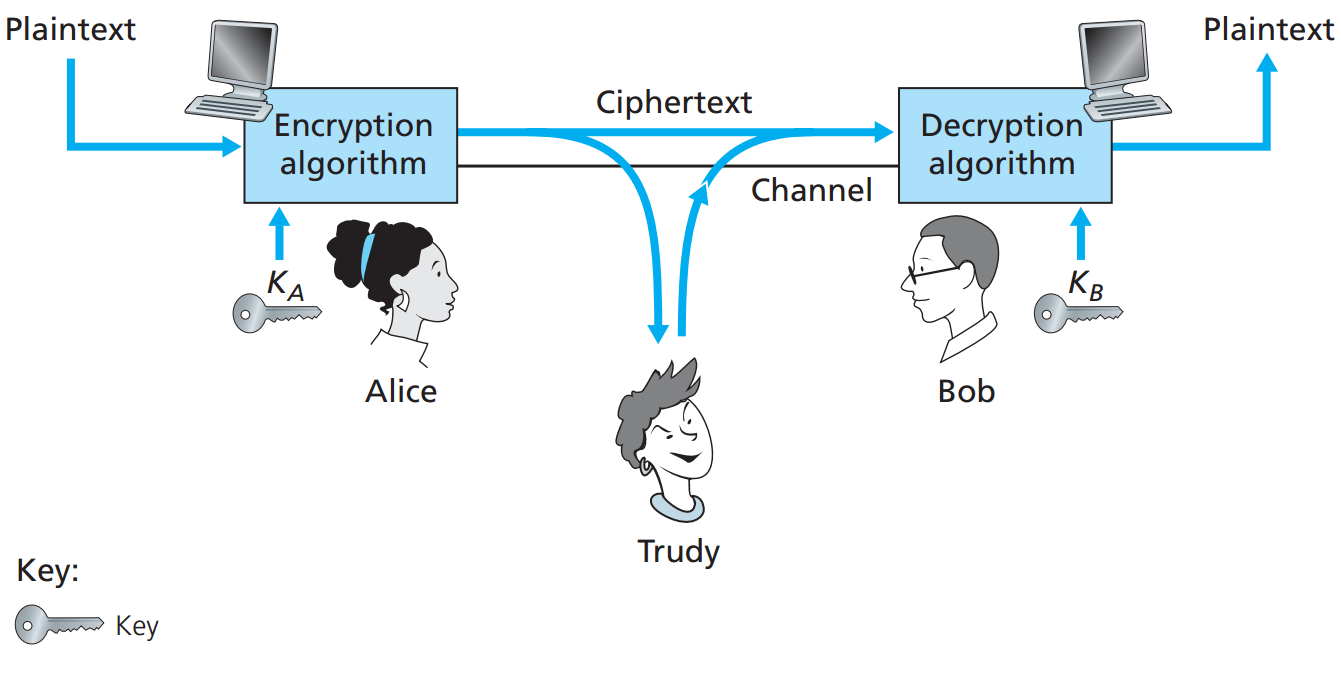
\includegraphics[width=14cm]{img/basic_crypto}}
  \caption[Basic cryptosystem diagram]{Basic cryptosystem diagram. Source: Kurose and Ross \cite{kurose2010computer}.}
  \label{fig:cryptoflow}
\end{figure}


It is assumed at all times that Eve has access to the communication lines, and can always know the ciphertext that is being sent between Alice and Bob. It is also a good practice to assume that the encryption and decryption algorithms are known to Eve, which leaves the key as the most important part of the scheme. As mentioned previously, Alice and Bob need to establish the means to agree on a private key, without anyone else knowing what this key is. As soon as the key is known to the attacker, i.e. Eve, all further communication is compromised. When that happens, another key has to be chosen and agreed upon once more by Alice and Bob.

The nature of the encryption and decryption can be classified in two broad categories: symmetric and asymmetric key encryption. Agrawal \cite{CryptoKeys} describes both categories by looking at the keys used. In \textbf{symmetric encryption}, the key used for encryption is virtually the same used in decryption. Therefore, key distribution has to be done before the tranmission of the messages. The key length has a direct impact on the security offered by the encryption algorithm. Meanwhile, \textbf{asymmetric encryption} employs two different keys: public and private. The public key is closely tied to the receiver, and it is used for encryption of the data. It is called public because it is available for general use; therefore, Alice can use Bob's public key to send him messages. On the other hand, the private is kept secret from the outside world, and is only available by an authorized person. The public and private keys always come in pairs, and this is because while the public key is used to encrypt data; its counterpart, the private key, is used to decrypt the data. 

\section{Introduction to Number theory}

In other to understand more topics pertaining cryptosystems, number theory and its notation, as well as some relevant theorems must be introduced. According to Stark \cite{stark1970introduction}, number theory consists of the study of the properties of whole numbers, and it is considered to be inextricably linked to cryptography. Goodrich \cite{2008algorithm} introduces number theory and most of its relevant aspects, most of which is briefly summarized as follows.

\subsection{Fundamental Theorems}

Given positive integers $a$ and $b$, we use the notation 
\[
a|b
\]
to indicate that $a$ \textbf{divides} $b$, that is, $b$ is a multiple of $a$. If $a|b$, then we know that there is some integer $k$, such that $b=ak$. From this definition, the following properties are found:

\begin{theorem}
  \emph{(Theorem on Divisibility)} Let a, b and c be arbitrary integers,
  \begin{itemize}
  \item If $a|b$ and $b|c$, then $a|c$.
  \item If $a|b$ and $a|c$, then $a|(ib+jc)$, for all integers $i$ and $j$.
  \item If $a|b$ and $b|a$, then $a=b$ or $a= -b$.
  \end{itemize}
\end{theorem}

An integer $p$ is said to be \textbf{prime} if $p\geq 2$ and its only divisors are the trivial divisors $1$ and $p$. Therefore, in the case $p$ is a prime, $p|q$ implies $d=1$ or $d=p$. An integer greater than 2 that is not prime is said to be \textbf{composite}. Also, two integers which only share a common divisor of 1 are considered to be \textbf{relatively prime}.


\begin{theorem}
\emph{(Fundamental Theorem of Arithmetic)}
Let $n > 1$ be an integer. Then there is a unique set of prime numbers $\{p_{1}, \dots p_{k}\}$ and positive integer exponents  $\{e_{1}, \dots , e_{k}\}$, such that

\[
n = p_{1}^{e_{1}} \cdots p_{k}^{e_{k}}
\]
\end{theorem}

The above product $p_{1}^{e_{1}} \cdots p_{k}^{e_{k}}$ is the prime decomposition of $n$. In other words, any positive integer is made up of the product between two prime numbers.   

\subsection{Modular Arithmetic}

The remainder of $a$ when divided by $n$ is expressed as $a \mod n$, that is:

\[
  r = a \Mod{n}
\]

\noindent which means that there is some integer $q$, such that

\[
  a = qn + r
\]

The remainder $r$ is resulting from $a \mod n$ is always an integer in the set $\{0, 1, 2, \dots, n-1\}$, even when $a$ is negative. The integer $n$ is called the \textbf{modulus}. 

\textbf{Congruence} modulo $n$ is a relevant concept to mention as well. If
\[
  a \Mod{n} = b \Mod{n},
\]
\noindent then we say that $a$ is \textbf{congruent} to $b$ modulo $n$, so it can be written in this way:
\[
a \equiv b \pmod n
\]
Therefore, if $a \equiv b \mod n$, then $a-b=kn$ for some integer $k$. 

Congruences have the following properties: 
\begin{enumerate}
\item $a \equiv b \pmod n$ if $n|(a-b)$.
\item $a \equiv b \pmod n$ implies $b \equiv a \pmod n$.
\item $a \equiv b \pmod n$ and mod $b \equiv c \pmod n$  imply $a \equiv c \pmod n$.
\end{enumerate}

Suppose that there is a mapping of all integers by the $\pmod n$ operator into the set of integers $\{0, 1, \dots, (n-1)\}$. The technique used to perform arithmetic operations within the confines of this set is known as \textbf{modular arithmetic}. Modular arithmetic exhibits the following properties:

\begin{enumerate}
\item $[(a \Mod{n}) + (b \Mod{n})] \Mod{n} = (a + b) \Mod{n}$
\item $[(a \Mod{n}) - (b \Mod{n})] \Mod{n} = (a - b) \Mod{n}$
\item $[(a \Mod{n}) \times (b \Mod{n})] \Mod{n} = (a \times b) \Mod{n}$
\end{enumerate}
And so, the rules for ordinary arithmetic invoving addition, subtraction, and multiplication carry over into modular arithmetic, except that the result is always within the boundaries of the defined set, which is between 0 and $n-1$.

Having explained modulo operation, as well as a having introduced modular arithmetic operations, a very convenient notation, called the set of residues, can be now described. Let $Z_{n}$ denote the set of nonnegative integers less than $n$:
\[
Z_{n} = \{0,1,\cdots, (n-1)\}
\]

The set $Z_{n}$ is also called the set of \textbf{residues}, or \textbf{residue classes} modulo $n$, because if $b=a \mod n$, $b$ is sometimes called the \textbf{residue} of $a$ modulo $n$. The notation $Z_{n}$ represents the integers between 0 and $n-1$. Thus, when it says that ``Let $a$ be a member of $Z_{n}$'', it really means the same thing as ``Let $a$ be an integer between 0 and $n-1$.''

Modular arithmetic in $Z_{n}$, where operations on the elements of $Z_{n}$ are performed mod $n$, show properties similar to those in traditional arithmetic, such as the \textbf{associativity}, \textbf{commutativity}, \textbf{distributivity} of addition and multiplication, and the existence of \textbf{identity} elements 0 and 1 for addition and multiplication, respectively. However, other operations such as division and exponentiation, behave very differently than they do for normal arithmetic. 

Every element $x$ in $Z_{n}$ has an \textbf{additive inverse}, that is, for each $x \in Z_{n}$, there is a $y \in Z_{n}$ such that $x + y \mod n = 0$. In other words, it means there is an element $a'$ that multiplies $a$ modulo $n$ which equals 1.  A \textbf{multiplicative inverse} of $x$ is an element $z^{-1} \in Z_{n}$ such that $xx^{-1} \equiv 1 \mod n$. As well as in regular arithmetic, 0 does not have a multiplicative inverse in $Z_{n}$. There are some nonzero elements that do not have a multiplicative inverse in $Z_{n}$. However, for every $n$ that is prime, every element $x \ne 0$ of $Z_{n}$ has a multiplicative inverse.

\subsection{Order and Generators}

Given a prime $p$ and an integer $a$ between 1 and $p-1$, the \textbf{order} of $a$ is the smallest exponent $e > 1 $ such that
\[
  a^{e} \equiv 1 \mod q
\]

A \textbf{generator}, or primitive root, of $Z_{p}$ is an element $g$ of $Z_{p}$ with order $p-1$. It is called a generator, because the repeated exponentiation of it can generate all the elements in $Z_{p}^{*}$. $Z_{p}^{*}$ is a subset of $Z_{p}$, defined to be the set of integers between 1 and $n$ that are relatively prime to $n$. 

\begin{theorem}
\emph{(Theorem on generators)}
If $p$ is a prime, then set $Z_{p}$ has $\phi(p-1)$ generators.
\end{theorem}

\subsection{Other Relevant Points on Modular Arithmetic}

%\item 
\begin{theorem}
\emph{(Fermat's Little Theorem)}
Let $p$ be a prime, and let $x$ be an integer such that \\ $x \mod p \ne 0$. In other words, that $p$ does not divide the integer $x$. Then
\[
x^{p-1} \equiv 1 \pmod{n}
\]
\end{theorem}

%\item 
\begin{theorem}
\emph{(Euclid's Division Theorem)} For every integer $m$ and positive integer $n$, there exist unique integers $q$ and $r$ such that $m=nq+r$ and $0 \leq r < n$. By definition, $r$ is equal to $m \mod n$.
\end{theorem}

Cliff and Ken \cite{cs21math19notes} review several important concepts regarding modular arithmetic, and are thus listed as follows:

\begin{itemize}
\item \textit{Adding multiples of n does not change values mod n}. That is, \\ $i \mod n= (i+kn) \mod n$ for any integer $k$.

\item Mod (by $n$) can be taken anywhere in calculation, as long as mod $n$ is taken from the final result.

\item \textit{Commutative, associative, and distributive laws}. Addition and multiplication mod $n$ satisfy the commutative and associative laws, and multiplication distributes over addition.

\item The expression ``$x \in Z_{n}$'' is used to mean that $x$ is a variable that can take on any of the integral values between 0 and $n-1$.
\end{itemize}

\section{Abstract Algebra: Groups and Rings}

Stallings \cite{CryptoStallings} describes groups and rings as some of the fundamental elements of a branch of mathematics known as abstract algebra. In abstract algebra, the focus is mostly on those elements that can be operated algebraically; in other words, how two elements of a set can be combined to obtain a third element in the set. The nature of the set is defined by the operations that can be performed on the elements of the set. It has been chosen that, by convention, the two main classes of operations on set elements are usually the same as the notations for addition and multiplication on traditional arithmetic. However, there is not really a limitation on the kind of operations that can be defined using abstract algebra.

\subsection{Groups}

A \textbf{group} G, denoted by $\{ G, \cdot \}$ is a set of elements with a binary operation, which is denoted by the operator $\cdot$. This operator is generic, and can refer not only to multiplication, but also to addition or some other mathematical operation. It associates to each ordered pair $(a, b)$ of elements in G an element $(a \cdot b)$ in G, such that the following axioms are followed:
\begin{description}
  \item[(A1) Closure:] If $a$ and $b$ belong to $G$, then $a \cdot b$ is also in $G$.
  \item[(A2) Associative:] $a \cdot (b \cdot c) = (a \cdot b) \cdot c $ for all $a$, $b$, $c$ in $G$.
  \item[(A3) Identity element:] There is an element $e$ in $G$ such that $a \cdot e = e \cdot a = a$ for all $a$ in $G$.
  \item[(A4) Inverse element:] For each $a$ in $G$ there is an element $a'$ in G such that $a \cdot a' = a' \cdot a = e$ 
\end{description}
It is worth noting that if a group has a finite number of elements, it is called a \textbf{finite group}, and the order of the group is equal to the number of elements in the group. Otherwise, the group is an \textbf{infinite group}. Moreover, a group is said to be \textbf{abelian} if it satifies the following condition, known as the commutative property:
\begin{description}
  \item[(A5) Commutative] $a \cdot b = b \cdot a$ for all $a$, $b$ in $G$.
\end{description}

When the group operation is addition, the identity element is 0; the inverse element of $a$ is $-a$; and subtraction is defined with the following rule: $a-b = a+(-b)$. 
  
\subsection{Rings}

A \emph{ring} $R$, which is sometimes denoted by $\{R, +, \times \}$, is a set of elements with two binary operations, called \textit{addition} and \textit{multiplication}, such that for all $a$, $b$, $c$ in $R$, there are some axioms that must be obeyed. It must be pointed out that a ring fulfills the same axioms as an abelian group with respect to addition; that is, axioms A1 through A5. The rest of the axioms obeyed by a ring are listed as follows:
\begin{description}
\item[(M1) Closure under multiplication:] If $a$ and $b$ belong to $R$, then $a \times b$ is also in $R$.
\item[(M2) Associativity of multiplication:] $a(b \times c) = (a \times b)c$ for all $a$, $b$, $c \in R$.
\item[(M3) Distributive laws:] $a(b+c) = (a \times b) + (a \times c)$ for all $a$, $b$, $c$ in $R$. \\ $(a+b)c = (a \times c) + (b \times c)$ for all $a$, $b$, $c$ in $R$.
\end{description}

Essentially, a ring is a set in which addition, subtraction $[a-b = a + (-b)]$, and multiplication can be done without leaving the set. Furthermore, a ring is said to be \textbf{commutative} if it satisfies the following additional condition:
\begin{description}
\item[(M4) Commutativity of multiplication:] $ab = ba$ for all $a$, $b$, $c$ in $R$.
\end{description}

Additionally, there are other axioms that, if obeyed, turn the commutative ring into an \textbf{integral domain}. The axioms are:  

\begin{description}
\item[(M5) Multiplicative identity:] There is an element 1 in $R$ such that $a1 = 1a = a$ for all $a$ in $R$.
\item[(M6) No zero divisors:] If $a$, $b$ in $R$ and $ab=0$, then either $a=0$ or $b=0$.
\end{description}

\subsection{Homomorphisms}

As it has been previously noted, operations within a closed group always result in another element from the group. Only one operation is allowed in a group: addition or multiplication, for instance. There may also be two groups or sets that are made up of different elements, each with its own operation. A \emph{homomorphism} consists of the construction of a function that \emph{translates} elements from one group to another group with the same properties.

\subsubsection{Group homomorphism}

According to Beachy and Blair \cite{beachy2006abstract}, a homomorphism is defined as follows: Let $G_{1}$ and $G_{2}$ be groups, and let $\phi: G_{1} \rightarrow G_{2}$ be a function. Then $\phi$ is said to be a \textbf{group homomorphism} if
\[
\phi(a*b) = \phi(a) *' \phi(b)
\]
for all $a$, $b$ in $G_{1}$.

Consider the example presented by Sorzano \cite{sorzano2013}, where there are two sets: $S= \{a, b, c\}$ and $S' = \{A, B, C\}$  with the operations $*: S \times S \rightarrow S$ and $*' : S' \times S' \rightarrow S'$. The operations within each group map two elements to another element from the same group. For example, $b*c=a$ and $a*a=a$, and in the other group, $A*A = A$ and $B*C=A$. So it can be seen that there is some similarity in the nature of the operations from both groups. Now consider the homomorphism between both groups, where:
\[
\begin{split}
  \phi: S \rightarrow S' \\
  \phi(a) = A \\
  \phi(b) = B \\
  \phi(c) = C \\
\end{split}
\]

\noindent Therefore, the following holds true using the above homomorphism:

\[
b*c=a \rightarrow \phi(b) *' \phi(c) = \phi(a) \rightarrow B *' C = A
\]

What this means is that a homomorphism serves as a link to translate operations from one group to the other, keeping the same properties.

\subsubsection{Ring Homomorphism}

Similarly to groups, there are also homomorphisms for rings, the main difference being that, instead of a single operation, two operations are considered.

Let $R$ and $S$ be rings with addition and multiplication. The map $\phi: R \rightarrow S$ is a homomorphism if:
\begin{enumerate}
\item $\phi$ is a group homomorphism on the additive groups $(R, +)$ and $(S,+)$
\item $\phi(xy) = \phi(x) \phi(y)$ $\forall x, y \in R$
\end{enumerate}

\section{Homomorphic Encryption}

Homomorphic is a word that has its roots in Greek, and it means ``the same shape''. It is used in various areas, such as abstract algebra, which then inspired its use in cryptography. This concept refers to the ability to make computations, i.e. operations such as addition and multiplication, on encrypted data without sharing the secret key to decrypt the data prior to the computations. 

Before homomorphic encryption, any change to the secret value contained in a ciphertext required the corresponding secret key, so that it could be decrypted, applied the change, and re-encrypted. However, homomorphic encryption eliminates the need of sharing the secret key, especially with those that are not to be completely trusted, in the event that there is some change that must be applied to encrypted data. 
Lange \cite{lange2011} mentions several applications that would benefit from a homomorphic encryption function, given its ability to manipulate encrypted data. Such applications fall in the domain of: e-cash, e-voting, private information retrieval (encrypted databases), and cloud computing.

\subsection{What is Homomorphic Encryption?}
According to P{\"o}tzelsberger \cite{potzelsberger2013kv}, when the encryption function of a cryptosystem is a homomorphism, meaning that it preserves group operations performed on ciphertexts, it is called a \emph{homomorphic cryptosystem}. The group operation considered for this kind of cryptosystem is either the arithmetic addition or multiplication, or both. A homomorphic encryption is additive if:

% a \textit{homomorphic cryptosystem} is a cryptosystem which encryption function is a homomorphism, and thus preserves group operations performed on ciphertexts.
% Either arithmetic addition or multiplication is the group operation considered.  

\[
\mathcal{E}(x+y) = \mathcal{E}(x)\otimes \mathcal{E}(y)
\]

where $\mathcal{E}$ denotes an encryption function, $\otimes$ denotes an operation depending on the used cipher and $x$ and $y$ are plaintext messages. A homomorphic encryption is multiplicative if:

\[
\mathcal{E}(x \cdot y) = \mathcal{E}(x) \otimes \mathcal{E}(y)
\]

where again $\mathcal{E}$ denotes an encryption function, $\otimes$ denotes an operation depending on the used cipher and $x$ and $y$ are plaintext messages.

The above conditions denote that the result of the operations between both inputs, in this case $x$ and $y$, is going to be the same whether the operations are performed after or before encryption. This property is what makes it possible to perform computations on an encrypted value which later can be decrypted to the correct result.

\subsection{Classification of Homomorphic Encryption Schemes}

Homomorphic encryption schemes are classified in two broad groups, depending on how they are defined, namely: partially homomorphic and fully homomorphic. 

\textit{Partially homomorphic encryption} schemes are defined over a group, and they support one operation at most: either addition or multiplication. On the other hand, \textit{fully homomorphic encryption} schemes are defined over a ring, and can support up to two operations: addition and multiplication.

According to P{\"o}tzelsberger \cite{potzelsberger2013kv}, even though somewhat homomorphic cryptosystems support a limited number of homomorphic operations, they are the building blocks for fully homomorphic encryption, and provide much more efficiency and shorter ciphertexts than their fully homomorphic counterparts. 


\subsection{Explaining Homomorphic Encryption}

Craig Gentry \cite{homoenc} explains the concept behind homomorphic encryption in a very simple way. Imagine that Alice has a jewelry store and wants her workers to assemble raw materials (diamonds, gold, silver, etc.) into finished products (necklaces, rings, etc.), but does not trust them, thinking they might run off with the raw materials at their first chance. So instead of giving them direct access to the materials, Alice places the materials inside a transparent glove boxes, which are then promptly locked with a key that only Alice has. This way, workers can put their hands inside the gloves that are connected to the box, and through them, work with the raw materials. Additionally, the workers are able to put in things inside the boxes, such as soldering iron to use on the raw materials, even though they cannot take anything out of it, since they do not have the key to open the box. Once the products are finished, Alice can then recover the products from the box using her key. The analogy is not perfect, because the workers are able to see the materials while working on them, but it is relevant because homomorphic encrytion means that they cannot take the materials with them.

Hayes \cite{Hayes2012} offers a proof of concept that accurately describes the very essence of a homomorphic cryptosystem. It is shown as follows: consider that the plaintext consists of integers; to encrypt a number, double it; to decrypt it, divide by 2. Using this scheme, addition and a nonstandard version of multiplication can be done on the encrypted data. Given the plaintext inputs $x$ and $y$, we can encrypt each of them separately, add the ciphertexts, and finally decrypt the result. This calculation would give the correct answer, expressed as $2x+2y=2(x+y)$. In other words, it is the same result as if each plaintext input were multiplied separately and then added with each other, because in the end, dividing it by two causes the same effect on both sides. 
Regarding multiplication, a little tweak has to be done for it to work. The product of the ciphertexts is defined as $(\frac{1}{2}) C_x C_y$, while the plaintexts are multiplied by the regular formula $xy$. 
As an example, consider $x=5$ and $y=7$. The result of the multiplication would come as $x \times y = 35$. To perform the same evaluation between ciphertexts, both inputs would be encrypted following the rule previously defined:
\[
C_{x} = 5 \times 2 = 10
\]
\[
C_{y} = 7 \times 2 = 14
\]
The multiplication is performed as $(\frac{1}{2}) 10 \times 14 = 70$, and it is divided by 2 to decrypt the ciphertext: $\frac{70}{2} = 35$, which turns out to be the correct result of the multiplication.

Certainly, the above cryptosystem is considered to be \emph{fully homomorphic}, since it supports both addition and multiplication. However, it is definitely not a secure one, since anyone that knows of the workings of the cipher can easily get to learn the secret message. This is also partly the reason of why the encryption and decryption algorithms are not usually kept as a secret, because it would be quite impractical to make a different encryption and decryption algorithm every time it were discovered. 

Stuntz \cite{stuntz2010} provides an example of a cipher scheme that has an inherent homomorphic property. Consider the popular, yet insecure, ROT13 cipher, also known as the Caesar cipher. The ROT13 is a simple substitution cipher which changes each letter with the letter that is thirteen positions ahead on encryption. To do decryption, it does the opposite: each character goes back thirteen positions in the alphabet. 
ROT13 is partially homomorphic with respect to the concatenation operation, because it is possible to concatenate two different pieces of ciphertexts. At decryption, the concatenation of the two pieces of ciphertexts ends up to be same as the concatenation of the original messages, the plaintext. Therefore, it is partially homomorphic with respect to concatenation. 

Consider, for instance, the plaintext pair $P_{1}=$ HELLO and $P_{2}=$ WORLD, which both concatenate to ``HELLOWORLD''. If both plaintexts were encrypted using ROT13, the ciphertexts would be $C_{1}=$ URYYB and $C_{2}=$ JBEYQ, and if concatenated, ``URYYBJBEYQ''. Therefore, if the result of the ciphertext concatenation were decrypted, it would result in ``HELLOWORLD'', which is exactly the same message obtained when the pair of plaintexts were concatenated originally. Figure \ref{fig:homosample} shows the aforementioned example as it goes through the encryption and decryption processes. 

\begin{figure}[H]
  \centerline{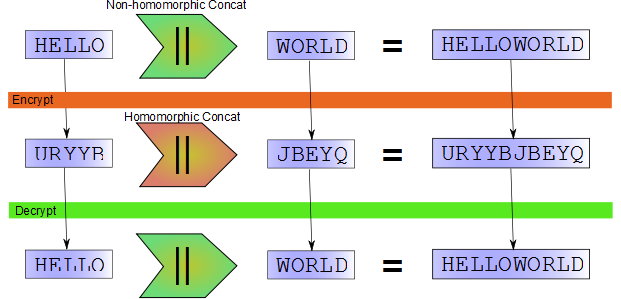
\includegraphics[scale=0.5]{img/rot13homo}}
  \caption[Example of the homomorphic property in ROT13]{Example of the homomorphic property in ROT13. Source: Stuntz \cite{stuntz2010}.}
  \label{fig:homosample}
\end{figure}

\subsection{The First Fully Homomorphic Encryption Scheme}

In an article published by the research staff of the NSA \cite{NSA2014}, it is discussed how the term of fully homomorphic encryption has been around for about 30 years, and only recently, in 2009 to be exact, a very important breakthrough regarding fully homomorphic encryption was made by Craig Gentry. Thanks to this breakthrough, the first fullly homomorphic scheme was created, opening the doors of research to this topic that was thought to be at a dead end. 

As Gentry \cite{homoenc} himself points out, by ``fully'' it means that there are no limitations on what manipulations can be performed on the ciphertext. Given ciphertexts $c_{1}, \dots, c_{t}$ that encrypt $m_{1}, \dots, m_{t}$ with a fully homomorphic encryption scheme under some key, and given any efficiently computable function $f$, anyone can efficiently compute a ciphertext (or set of ciphertexts) that encrypts $f(m_{1}, \dots, m_{t})$ under that key. This permits all kinds of computations on the encrypted data. Of course, no information about the plaintexts $m_{1}, \dots, m_{t}$ or the value of $f(m_{1}, \dots, m_{t})$ is leaked. 

The first step in Gentry's blueprint was to construct a \emph{somewhat homomorphic encryption scheme} (SWHE), which was capable of evaluating ``low-degree'' polynomials homomorphically. In order to obtain a fully homomorphic encryption scheme, Gentry proposed a \emph{bootstrapping theorem} which made it possible to transform the original somewhat homomorphic encryption scheme into a \emph{leveled} fully homomorphic encryption one.

One of the main problems that fully homomorphic encryption faces is the managing of ``noise'' in the ciphertext. In this case, noise refers to the gradual distortion of ciphertexts that is caused by doing operations (e.g., addition or multiplication) on them. As more operations are performed on the ciphertext, the larger the noise becomes, rendering the ciphertext undecipherable, as it would end up with the wrong result after attempting to decrypt. As Hayes \cite{Hayes2012} points out, each homomorphic addition doubles the noise, and each multiplication squares it. Thus, the number of operations must be limited, should one not wish to ``corrupt'' the ciphertext. 

An obvious solution to the problem of accumulating noise is to decrypt the data and re-encrypt it whenever the noise begins to approach the critical threshold. Thus, the noise is resetted to its original level, allowing for more operations. The problem with this approach is that decryption needs the secret key, which is usually not going to be available to whoever is performing the operations on the ciphertext. 

Instead, Gentry developed a process called \emph{bootstrapping} to overcome the problem of noise accumulation. The \emph{evaluate} function used in the cryptosystem can virtually perform any computation, as long as it has not reached the critical threshold of noise. Therefore, that very function is used to run the \emph{decrypt} function, which takes as input the noise-heavy ciphertext that has gone through several operations, and the \emph{encrypted secret key}. This makes sense because the decrypt function relies on the evaluate function, which was made to work on encrypted values. So when the \emph{decrypt} function is run, the decrypted result is not the plaintext, but rather a new encryption, with reduced noise. This process of re-encrypting and refreshing the noisy ciphertext can be repeated as many times as needed, because then it technically has no limitations on the number of operations it can perform. However, extra layer of encryption will consequently increase the overall computational effort required to complete the set of operations desired to be performed. As the research staff from the NSA exemplifies \cite{NSA2014}, if the process were to be used by Google to search the web homomorphically, the normal computing time required would be multiplied by about a trillion. This is the reason why this scheme is not practical enough as a solution for implementation.

\subsection{Learning with Error Problems}

Some problems are considered \emph{hard} to solve, meaning that no polynomial time algorithm is known. However, this is a good thing in cryptography, since data encryption relies on the computational difficulty to solve problems. As the slides by Sahni \cite{sahni1999} point out, many modern cryptosystems rely on the difficulty of these problems, such as RSA and Elliptic Curve Cryptography.

Blum \cite{Blum:1993:CPB:646758.759585} suggests that learning problems have certain properties which make them possible sources of cryptographic hardness. Two of these problems are the learning with errors problem, and its variation, the ring-learning with error problem.

The learning with errors (LWE) problem was introduced by Regev \cite{Regev:2005:LLE:1060590.1060603}; it is defined as follows:

\theoremstyle{definition}
\begin{definition}
{Learning with Errors Problem}
For security parameter $\lambda$, let $n = n(\lambda)$ be an integer dimension, let $q=q(\lambda) \geq 2$ be an integer, and let $\chi = \chi(\lambda)$ be a distribution over $\mathbb{Z}$. The LWE $(n, q, \chi)$ problem is to distinguish the following two distributions: In the first distribution, one samples $(a_{i},b_{i})$ uniformly from $\mathbb{Z}_{q}^{n+1}$. In the second distribution, one first draws $s \leftarrow \mathbb{Z}_{q}^{n}$ uniformly and then samples $(a_{i}, b_{i}) \in \mathbb{Z}_{q}^{n+1}$ by sampling $a_{i} \leftarrow \mathbb{Z}_{q}^{n}$ uniformly, $e_{i} \leftarrow \chi$, and setting $b_{i} = \left \langle a,s  \right \rangle + e_{i}$. The LWE $(n, q, \chi)$ assumption is that the LWE $(n, q, \chi)$ problem is infeasible.
\end{definition}

Regev proved that for certain moduli $q$ and Gaussian error distributions $\chi$, the LWE $(n, q, \chi)$ assumption is true as long as certain worst-case lattice problems are hard to solve using a quantum algorithm. Later, Peikert \cite{Peikert:2009:PCW:1536414.1536461} de-quantized Regev's results, proving that the LWE $(n, q, \chi)$ assumption is true as long as certain worst-case lattice problems are hard to solve using a \emph{classical algorithm} as well.

At a later date, the ring learning with errors (RLWE) problem was introduced by Lyubaskevsky et al. \cite{rlwe2010}. The learning with errors (LWE) problem and the ring learning with errors (RLWE) problem are syntactically identical, aside from using different rings (the first one uses $\mathbb{Z}$ and the second one a polynomial ring). 

Regev \cite{regevlearning} gives a convenient definition of the ring-LWE problem. Let $n$ be a power of two, and let $q$ be a prime modulus satisfying $q=1 \mod 2n$. Define $R_{q}$ as the ring $\mathbb{Z}_{q}[X] / \left \langle x^{n} + 1 \right \rangle$ containing all polynomials over the field $\mathbb{Z}_{q}$ in which $x^{n}$ is identified with $-1$. In ring-LWE, we are given samples of the form $(a, b = a \cdot s + e) \in R_{q} \times R_{q}$, where $s \in R_{q}$ is a fixed secret, $a \in R_{q}$ is chosen uniformly, and $e$ is an error term chosen independently from some error distribution over $R_{q}$. The goal is to recover the secret $s$ from these samples (for all $s$, with high probability).

Because of the hardness and versatibility of both problems, they have become popular as the basis for cryptographic constructions. Regev \cite{regevlearning} notes that LWE has been used as the basis of public-key encryption schemes that are considered secure under chosen-plaintext attacks, chosen ciphertext attacks, oblivious transfer protocols, and more.

To understand how a LWE can be applied in cryptography, consider the following simple cryptosystem described by Regev \cite{regevlearning}, which is parameterized by integers $n$ (the security parameter), $m$ (number of equations), $q$ (modulus), and a real $\alpha > 0$ (noise parameter). One possible choice that guarantees both security and correctness is the following. Choose $q$ to be a prime between $n^2$ and $2n^2$, $m=1.1 \cdot n\log q$, and $\alpha = \dfrac{1}{\sqrt{n} \log^{2}n}$. All additions are performed modulo $q$ in the following description. 

\begin{itemize}
\item \textbf{Private key}: The private key is a vector $s$ chosen uniformly from $\mathbb{Z}_{q}^{n}$.
\item \textbf{Public key}: The public key consists of $m$ samples $(a_{i}, b_{i})_{i=1}^m$ from LWE distribution with secret $s$, modulus $q$, and error parameter $\alpha$.
\item \textbf{Encryption}: For each bit of the message, choose a random set $S$ uniformly among all $2^m$ subsets of $[m]$. The encryption is $(\sum_{i \in S} a_{i}, \sum_{i \in S} b_{i})$ if the bit is 0 and $(\sum_{i \in S} a_{i}, \left \lfloor{\frac{q}{2}}\right \rfloor + \sum_{i \in S} b_{i})$ if the bit is 1.
\item \textbf{Decryption}: The decryption of a pair $(a,b)$ is 0 if $b - \left \langle a,s \right \rangle$ is closer 0 than to $\left \lfloor \frac{q}{2} \right \rfloor$ modulo $q$, and 1 otherwise. 
\end{itemize}
Such a cryptosystem is quite inefficient, but it serves its purpose to establish a link between the LWE problem and its use in cryptography.

Hayes \cite{Hayes2012} writes in his article that recently, Brakerski, Vaikuntanathan and Gentry have developed a variant of the learning-with-errors system that takes a different approach to noise management. Instead of stopping the computation at intervals to re-encrypt the data, they incrementally adjust parameters of the system after every computational step in a way that prevents the noise level from ever approaching the limit.

\subsection{Brakerski-Gentry-Vaikuntanathan Scheme}

The Brakerski-Gentry-Vaikuntanathan (BGV) scheme \cite{cryptoeprint:2011:277} is a leveled fully homomorphic encryption that does not rely on bootstrapping, but rather employs it as an optimization. However, it still follows Gentry's blueprint to build a fully homomorphic cryptosystem, thus lattice-based cryptography is employed, albeit with certain improvements. It is described as \emph{leveled} in the sense that the parameters of the scheme depend (polynomially) on the depth of the circuits that the scheme is capable of evaluating.

This scheme dramatically improves performance compared to previous attempts at fully homomorphic encryption, and also bases security on weaker assumptions. The security of the BGV scheme is based on the ring-learning with error (RLWE) problem that has a $2^{\lambda}$ security against known attacks.

As it happens with the first fully homomorphic encryption scheme proposed by Gentry \cite{homoenc}, making computations on the ciphertext creates a noise that gradually accumulates. Specifically, performing one addition between two ciphertexts roughly doubles the noise, while multiplication squares it. Decryption succeeds as long as the magnitude of the noise does not surpass a certain threshold. However, the BGV scheme proposes a \emph{noise-management technique} that keeps the noise in check by reducing  it after doing homomorphic operations, without depending on the bootstrapping technique previously mentioned. The noise management technique is called \emph{modulus switching}, and it was developed by Brakerski and Vaikuntanathan \cite{cryptoeprint:2011:344}, albeit with a modification. 

The lemma that describes the original modulus-switching technique says that an evaluator who does not know the secret key $s$, but instead only knows a bound on its length, can transform a ciphertext $c$ modulo $q$ into a different ciphertext modulo $p$ while preserving correctness. This is expressed as $[\left \langle c',s \right \rangle]_{p} = [\left \langle c,s  \right \rangle]_{q} \mod 2$. The interesting property found here is that if $s$ is short and $p$ is sufficiently smaller than $q$, then the ``noise'' in the ciphertext actually decreases, meaning that $|[\left \langle c',s \right \rangle]_{p}| < |[\left \langle c,s \right \rangle]_{q}|$. This technique allows the evaluator to reduce the magnitude of the noise without knowing the secret key, and without depending on bootstrapping. The BGV scheme takes the aforementioned technique, and further improves noise management by making use of a \emph{ladder of gradually decreasing moduli}.  

This homomorphic scheme has been implemented as a software library in C++, called HElib \cite{helib}. The implementation focuses on the effective use of the Smart-Vercauteren ciphertext packing techniques and the Gentry-Halevi-Smart optimizations. Halevi and Shoup \cite{cryptoeprint:2014:106} describe in a paper the algorithms employed on the implementation, as well as some considerations to have in mind depending on the hardware used.

\subsection{Applications}

As it was previously mentioned, various individuals and corporations are hesitant to make use of cloud services, mainly because of the security risks it poses, such as privacy loss and tampering of the data. Traditional cryptosystems can protect confidentiality if the only goal is remote storage; but it is restricted to just that. However, if the encryption employed were homomorphic, the cloud server where the data is stored would be able to perform meaningful computations on the encrypted data.  The scenarios where homomorphic encryption can be applied are many, and some of the most important areas are: medical applications, financial applications, advertising and pricing, electronic voting, data mining, and biometric authentication.

\begin{description}
\item[Medical applications.-] A straightforward application of homomorphic encryption in a medical context is the storage and processing of medical records of patients. Most of the time, these records are considered private, but a hospital would be greatly benefited if it could rely on a cloud service rather than setting up its own data center. If homomorphic encryption has been used as a cipher to protect the medical records, then there could be meaningful pieces of information that could be extracted from it. For example, if a doctor in another clinic was granted access to the patient's medical record, he could make use of a function that makes homomorphic evaluations on the encrypted record to obtain statistical data from the patient. And this would be possible without the cloud server learning what information the medical record contained.
\item[Financial applications.-] Data about corporations, such as their stock price, performance or inventory is often considered to be private, and also very relevant towards making investment decisions. There are many kinds of computations that could be done on this private data, such as running predictive simulations on stock price performance. 
\item[Advertising and pricing.-] Nowadaways, user activity is heavily monitored by the websites that he browses, and uses this data as to build a profile and direct to him appropriate ads. Take Amazon as an example: Amazon keeps a history on what items the user is looking at, even if they were not bought, for further advertising. The user might get emails advertising the same or similar products, or might even see the same ads on unrelated sites, such as Facebook \cite{KimMai}. 
  The above example is just the tip of the iceberg. There is a lot of contextual information that can be retrieved from the user to gain insight on his interests and current status, without him having to be active. For example, he could be suscribed to a service that sends alerts to his smartphone whenever he is walking nearby a shop that could be of his interest. Geolocation and user profile are pieces of information that are considered to be private, the user might not subscribe to the service if it just shared around his information. If, however, he is guaranteed that his information is being kept encrypted, and that it stays that way whenever a computation is made to see if there is a nearby store of his interest, then he might not be as reluctant to make use of the service. The applications on advertising using homomorphic encryption are diverse, because there are pieces of data that can be obtained passively, such as the user's geolocation or browsing habits.
\item[Electronic Voting.-] Although not necessarily related to cloud computing, electronic voting is another area where homomorphic encryption can make such voting scheme feasible and convenient. Voting could be done from anywhere as long as the participant is provided with Internet access. Simply put, homomorphic encryption can be used to hide the content of a ballot by calculating the total number of votes, without having to decrypt any of the ballots. However, electronic voting is not as trivial as it seems, because apart of confidentiality, there are other security parameters that are equally important, such as: correctness of the tally, democracy, robustness, verifiability, fairness, and verifiable participation. Therefore, applying homomorphic encryption would only satisfy one of the many requirements for electronic voting to be feasible.
\item[Data mining.-] Closely related to advertisement, data mining has several issues on privacy. Using homomorphic encryption would mean that certain sensitive attributes of customers data can be protected from unauthorized parties. Yang et al. \cite{YangZhongWright} have proposed a solution that allows a data miner to compute frequencies of values or tuples of values in the customers' data in a privacy preserving manner. The advantage of this solution is that, unlike other existing attempts to make data mining more private, is that this solution is both fully private and fully accurate, without compromising one in exchange of the other.
\item[Biometric Authentication.-] Biometric authentication is an area of application quite different from the rest. This is because biometric data is assumed to be public, since fingerprints virtually on every object touched by a person. Therefore, according to P{\"o}tzelsberger \cite{potzelsberger2013kv}, what is considered to be private is the relationship between the biometric data and the person from whom it comes. It can be applied on the scenario where the user tries to authenticate using one of his biometric features: the biometric feature would be stored and encrypted before it looks for a match in the database. The homomorphic evaluation would consist in the comparison between the user's biometric feature and all of the existing rows in the database. Traditional cryptographic would not be appropriate for this task, since biometric data can vary slightly each time, so an exact match would not work out. Assuming that the biometric feature is stored as a binary string, the homomorphic evaluation would consist in computing the Hamming distance between two feature vectors, and a predefined threshold to achieve the comparison. This is how the biometric data itself can stay public, but the relationship of whom it belongs to is kept private.
\end{description}

\section{Services in the cloud}

The cloud, a trendy term used to describe a network of servers usually accessible through the Internet, currently provides two important services: storage and computation. As Xu et al. in \cite{cryptoeprint:2011:574} point out, cloud storage services, such as Dropbox, Skydrive, Google Drive, and Amazon S3 have become very popular in recent years. As the use of these services become more common, more sensitive information is kept in the cloud, such as emails, health records, private videos and photos, company finance data, government documents, etc. 

Li et al. \cite{cryptoeprint:2009:593} introduce cloud computing as a new term that views computing as a utility which enables convenient, on-demand access to computing resources that can be rapidly deployed with minimal management overhead and great efficiency. Cloud computing has the potential to benefit its users in avoiding large capital expenditure used for deployment and management of both software and hardware, such as setting up a data center. 

All of these services are opening up a new era powered by the software as a service (SaaS) computing architecture. One of the main advantages of storing this information in the cloud is that the owners are relieved from the burden of data storage and maintenance at all times. There are many plans that adjust to the on-demand needs of the owner of the data, which is way less costly than building and maintaining a whole data center. This implies that the clients of these services can expect to gain reliability and availability from having the data stored remotely. On the other hand, the data is necessarily brought out of their control and protection. This becomes a risk for the owner of the data, since the information stored in the cloud could potentially be accessed by unauthorized individuals, such as competitors or malicious attackers. There also exists the possibility that the information stored could be tampered in some way, thus compromising its integrity. Therefore, the computing and storage service providers are usually not trusted completely, which is why it has been difficult for the public and organizations to fully adopt the use of these services.

The aforementioned issue brings up the need of having a mechanism that verifies that a cloud provider is storing the whole database intact, even the portions that are rarely accessed. Ateniese et al. \cite{cryptoeprint:2014:886} point out that, fortunately, a series of \textit{proofs-of-storage} protocols have been proposed to solve this problem related to data integrity. Xu et al. \cite{cryptoeprint:2014:395} define a proof of storage (POR or PDP) as a cryptographic tool, which enables a data owner or third party auditor to audit integrity of data stored remotely in a cloud storage server, without keeping a local copy of data or downloading data back during auditing. In other words, applying a proof of storage in a cloud server can guarantee that the data has not been tampered with; and in the event that it is, most likely the service could be held liable for damages to the data. A huge advantage of using a proof of storage is that the data does not have to be downloaded to confirm its integrity, which makes it ideal to make use of it routinely. 

One of the simplest use cases for cloud computing is when a user independent from the cloud wants to store some data in it for later retrieval. In this simple case, data confidentiality and integrity can be trivially ensured. For that, typical cryptography primitives can be used by encrypting the user's data before it is sent for storage in the cloud. To ensure confidentiality, the key used for encryption is kept secret from the cloud provider. However, real life applications are not as simple. Damgard et al. \cite{cryptoeprint:2013:629} mentions that the cloud is more than a storage medium; in particular, computation over the stored data is outsourced to the cloud. Sometimes it might even be distributed among distinct cloud servers geographically apart, operated by different parties. Wang et al. \cite{cryptoeprint:2009:081} describe the nature of the problem at length, because usually a cloud service is not solely restricted as a data warehouse. The data stored in the cloud may be frequently updated by the users, including insertion, deletion, modification, appending, reordering, etc. This kind of complex scenario is what makes the use of traditional cryptographic primitives so difficult to adapt, especially because the data is not stored in a single cloud server, but is instead redundantly stored in multiple physical locations to further reduce the data integrity threats. Therefore, making use of cloud services highly improve data avalability and storage flexibility, data confidentiality and integrity is put at risk.

In order to tackle these issues, there have been many attempts to make cloud services, especially cloud computing, more secure. These attempts are very different in nature, though very similar regarding its goals. These are \textit{secure multi-party computation} and \textit{homomorphic encryption}. David, Nishimaki, et al. \cite{cryptoeprint:2015:135} describes secure multiparty computation (MPC) as the means to allow mutually distrustful parties to compute functions on private data that they hold, without revealing data to each other. There are many methods and approaches proposed to perform secure multiparty computation, although only recent attempts are considered to be efficient enough for application. On the other hand, homomorphic encryption is based on the idea of performing computations on the ciphertext that has gone through an encryption algorithm, without having to decrypt it beforehand. This aspect makes homomorphic encryption a good technique for cloud services, since only the authorized users are able to decrypt the ciphertext after the necessary computations have been performed on it.

%Pendiente hacer un resumen del capitulo y ligarlo al siguiente capitulo

\clearpage

\chapter{Related Works}
\label{relatedWorks}

En este cap\'{\i}tulo se presentan cuatro trabajos relacionados con el sistema de detecci\'{o}n de reportes duplicados desarrollado en esta tesis. Se realiza una breve descripci\'{o}n de cada uno de los trabajos y se explican las similitudes y diferencias entre esos trabajos y este trabajo de tesis.

\clearpage

\chapter{Methodology}
\label{methodology}

The methodology in this work describes all the considerations and steps taken to build a solution to the problem analyzed from the case study. As such, the methodology has a very close relationship with the case study. The problem studied addresses a situation where a person stores sensitive data on the cloud, with the intention of accessing and modifying such data at a later time. The solution itself is an \emph{implementation of a client-server based software} that makes use of a library called HElib, which enables the use homomorphic encryption on integers.

Even though the object of study is the application of homomorphic encryption in the cloud, it is not trivial to find a fitting situation where it can be applied. The search becomes more complex as the limitations of state-of-the-art homomorphic encryption tools are considered. For example, it is fitting to pose a case study that is simple enough so that the currently available tools can be used effectively, and complex enough so that applying homomorphic encryption is compelling and better-suited than other alternatives.

This section discusses the case study and the means to offer a solution based on the cloud.  Then, it describes a proof of concept in a general way as a stand-alone solution. The tasks required for the proof of concept to work are briefly described, and some considerations regarding key management are noted. Afterwards, it mentions the scenario where a client-server architecture is employed, discussing some decisions that were made regarding the communication between the client and the server. Finally, it mentions how the aforementioned tasks are being split between each component.

\section{{Case Study}}

The case study considered for this work is explained as follows: commonly, a household has more than one member, e.g.\ partner and children. The responsible \emph{residents} (i.e.\ the parents) might want to keep an eye on the house while being away, especially if their children are left behind. They would like to ensure that their children stay inside during this time, and that nobody else, except for a babysitter, enters the house. And if it were the case that somebody got in or out, they would probably desire to be promptly notified of it. This holds true especially when they are away for long periods of time, during a vacation, for example. A traditional solution consists in setting up a surveillance system throughout the house, which would certainly work to prevent robbery, but wouldn't necessarily work as a measure to know whether or not the children have left the house. Additionally, such a system usually requires a monthly or yearly fee. Therefore, setting up a surveillance system might be too costly for some families, and not be quite adaptive to their needs. It might be more effective to deploy a system that detects when people enter and exit the building through the main doors, and keep a counter of it. 

The main idea is that the \emph{surveillance counter} initializes at some point in time, and, as people go in and out, the counter increases or decreases, respectively. Setting up the sensors and other pieces of hardware can be considered as a Do-It-Yourself project, as resources could easily be found. Wilson \cite{wilson2005simultaneous} mentions several considerations to take when tracking people inside a building using binary sensors. In this case, however, it is simpler to set it up, as it is not necessary to keep track of the people inside the building: only if they go in or out past the main doors. 

The issue comes out when the recorded data, that is, the counter, is to be accessed or modified securely over the web. 

\section{{Proposed Solution}}

The proposed solution addresses the issue hinted at the end of the case study description. The counter data that is recorded by the sensors is to be sent to a server somewhere in the cloud, where it will be stored indefinitely, awaiting for the data to be accessed or modified in the future. It might not be appropriate to have a dedicated server at home for this functionality, which is why the computing task is instead delegated to the cloud. The data stored in the cloud server can be accessed from anywhere else; however, one of the most important aspects of the whole scheme remains unaddressed: confidentiality.

Usually, the resident would not allow others to know about the actual counter, including the cloud server itself, as this information is considered to be \emph{sensitive}. The traditional approach is to make use of public-key cryptography to \emph{encrypt} the data and prevent from anybody else to know the counter. Once the counter data has been encrypted successfully, it can then be safely uploaded to the server in the cloud. Then, when the resident desires to view the value of the counter, he would have to download the data and \emph{decrypt} it in order to view it. This sounds reasonable until changes are applied to this value, since it would have to go again through the encryption process. Indeed, this would imply that every time there is a change in the counter, the whole ciphertext would have to be reuploaded to the server. Considering that a person comes in and out of a building quite frequently, it would turn out to be a heavy burden that carries an overhead cost, computational and bandwidth-wise, that keeps accumulating every time there is an update. 

An alternative approach is to simply notify the cloud service of any changes that occur, so that it performs the addition or subtraction itself instead of relying on receiving the whole encrypted result. Even though this would not be possible to do with traditional cryptography, it can be done using \emph{homomorphic cryptography}. The concept behind this approach is that, while the initial counter value is being stored on the server, the client part that resides on the household sends over any change of individuals that come in or out of the building. Thus, the cloud service performs the appropriate homomorphic computations on the currently stored value. This occurs without the need of reuploading the counter data, as the cloud service has no need of decrypting the data in the first place. Since the full ciphertext is not being re-sent, the overhead costs are reduced significantly.

Whenever the resident needs to know the value of the counter, he can authenticate with the cloud service to download the current ciphertext that represents the counter. The ciphertext can be decrypted using the private key generated at the beginning of the process. This aspect remains the same whether homomorphic encryption is used or not, and there is no way around it without compromising confidentiality. Considering that a system that detects when people come in and out might not be perfect, and if somehow the counter gets to an incorrect value, it could be reset to the correct amount by the user as required. In this case, it would be unavoidable to send a newly encrypted counter value.

The solution itself consists in an implementation of a client-server software that aims to store and modify securely a counter by making use of homomorphic encryption. The various tasks that help reach this goal are distributed by the client and server components of the software. The client focuses on the initialization of the homomorphic encryption scheme, generation of public and private keys, encryption of initial counter data, among other things. On the other hand, the server is dedicated to store and manage the public key of the household and its current counter value. Both parts of the software utilize a library called HElib, which makes it possible to run homomorphic evaluations. In other words, this library is used to perform basic operations on the data, such as addition, subtraction, and multiplication. Consequently, it is also used to generate the public and private keys, encrypt data, and decrypt it. Once the encrypted counter is stored in the server, a different kind of client, i.e.\ the resident, can then ask to download and decrypt it. It makes sense to say that it will be a different kind of client, since most likely the interested person would not be at the household, i.e., the place where the counter was initialized.

\section{{Details of the HElib library}}

An implementation of a homomorphic encryption scheme, the Brakerski-Gentry-Vaikuntanathan (BGV), is openly available as a C++ library, called HElib. Using this library, it is possible to encrypt integer values and perform operations on them while being encrypted. There are many parameters to be considered when using this implementation, and these usually define how the public and private keys are going to be like. For this particular application, most parameters can be left in their default values, as they seem to serve the intended purpose. 

Part of the description found in the code repository of HElib states that the library is considered to be low-level, and given its difficulty and constant changes, it is not fitting to build big applications with it. Regarding the use of the library and its implementation of homomorphic encryption, often referred to as \emph{HE}, the following is stated: ``At its present state, this library is mostly meant for researchers working on HE and its uses. Also currently it is fairly low-level, and is best thought of as \emph{assembly language for HE}. That is, it provides low-level routines (set, add, multiply, shift, etc.), with as much access to optimizations as we can give.'' Brakerski et al.\ \cite{helib}.

It is important to note that the library recently started to support multi-threading, which would considerably speed up the evaluation times of the homomorphic operations. Not too long ago it started to support bootstrapping as well, a technique that prevents the ciphertext from getting too much noise and that eventually results in the incorrect homomorphic evaluations.

\section{Setting up the Parameters and Context}

The HElib library is an implementation of a homomorphic encryption scheme, and as such, it has certain requirements before it can encrypt data or even generate keys. First of all, it has a list of parameters which must be manually set. Depending on the parameters applied, some aspects that directly affect the keys and ciphertext are altered. The suggested values are used for the majority of the parameters. Altering the values of the parameters could be an interesting way to do experimentation with the key size and computation time required.

Table \ref{tbl:parameters} briefly describes each parameter used in HElib. It does not go into much depth, as those details are mostly pertaining to the algorithms in the library.

\begin{table}[h]
  \caption{Parameters used in HElib}
  \label{tbl:parameters}
\centering
  \begin{tabular}{|l|l|l|}
    \hline
    \textbf{Parameter} & \textbf{Description} & \textbf{Value} \\ \hline
    R  &     number of rounds &  default=1     \\ \hline
    p  &     plaintext base  & default=2  \\ \hline
    r  &     lifting  & default=1  \\ \hline
    d  &     degree of the field extension  & default=1  \\ \hline
    c  &     number of columns in the key-switching matrices  & default=2  \\ \hline
    k  &     security parameter & default=80  \\ \hline
    L  &     number of levels in the modulus chain  & default=heuristic  \\ \hline
    s  &     minimum number of slots  & default=0  \\ \hline
    repeat &  number of times to repeat the test & default=1  \\ \hline
    m   &    use specified value as modulus & optional  \\ \hline
    mvec &   use product of the integers as  modulus & optional \\ \hline
    gens &   use specified vector of generators & optional \\ \hline
    ords  &  use specified vector of orders & optional \\ \hline
  \end{tabular}
\end{table}


\section{{Key Generation and Serialization}}

As the scheme implemented in HElib is based on public-key cryptography, it requires the use of public and private keys. The owner of the data has to generate his own set of keys as the first step, and it is only the public key which he should be willing to share. The user then shares his public key with the cloud service by some means of registration, so he does not have to share it every time he makes use of the service. The public key is used to encrypt the counter data for the first time before sending it over to the server, and the server itself requires this public key in order to perform any homomorphic operation.
The generation of the keys is pseudorandom, so extra care should be taken as to not use a predictable seed, so that the public and private keys are not recreated by another party. 

In order to generate a set of keys, a component called a \emph{context} needs to be instantiated using certain parameters. Firstly, the public key is obtained by simply instantiating an object of the class \textit{FHESecKey}. Then, a copy of the public key is made as the foundation for the private key. This exact copy applies a method called \textit{GenSecKey(w)}, which takes \textit{w} as a seed to create the real private key. Finally, it goes through a process that computes key-switching matrices, which are used in the internal algorithms of the library to create the secret key. The code for these actions are shown below:

\begin{lstlisting}[caption={Key generation},label={lst:keyGeneration},numbers=left,escapeinside={@}{@}]
  FHEcontext* context;
  FHESecKey* secretKey;
  FHEPubKey* publicKey;  
  context = new FHEcontext(m, p, r);
  // Set of keys are initialized
  publicKey = new FHESecKey(*context);
  secretKey = publicKey;
  // Secret key is fully created by using these two methods
  secretKey->GenSecKey(w); 
  addSome1DMatrices(*secretKey); 
\end{lstlisting}

Before proceeding to encrypt the data, it is important to have the public key serialized and ready to send it to the server. Serialization is a popular term used to describe the encoding of objects and the objects reachable from them, into a string of bytes. Serialization is a term introduced by Oracle \cite{oracleserial}, and it is commonly used for lightweight persistence and communication via sockets. In this case, it is used as the means of temporarily storing the public key in a stream of bytes so it can be shared with a remote server that will be able to read such stream. Only after the contents of the saved object have been fully read, it will be possible to reconstruct the public key. Fortunately, the HElib provides a very simple way to do serialization, since the class \textit{FHESecKey} supports the $\ll$ operator which works quite nicely with a couple popular serialization classes in C++ called \textit{istringstream} and \textit{ostringstream}. The use of this class is showed as follows: 

\begin{lstlisting}[caption={Key serialization},label={lst:serializeKey},numbers=left,escapeinside={@}{@}]
  ostringstream pkstream;
  pkstream << *publicKey;
\end{lstlisting}

As shown in Code Snippet \ref{lst:serializeKey}, the data stored inside the public key object has been stored as a stream of bytes in a highly portable object from the \textit{ostringstream} class. Using this newly populated object, the public key can be shared using sockets.

\section{{Encryption of the Counter Value}}

In order the protect the value of the counter from being known from other parties, including the server itself, it must be encrypted. This means that an encryption algorithm, provided by the HElib, is to be used on the plaintext that represents the counter. The result of this process is a \emph{ciphertext}, which, unless provided with the corresponding private key, cannot be deciphered back to its plaintext form. 

Following the conventions defined in the HElib, objects from the \textit{EncryptedArray} and \textit{PlaintextArray} are initialized using the \textit{context} and \textit{G} as parameters which were previously set. \textit{PlaintextArray} can be seen as a container for the plaintext, whereas \textit{EncryptedArray} is seen as a general container that works as an medium between the plaintext and ciphertext data. Once it has been done, a method called \textit{encode} of the same class can be used on the PlaintextArray object to prepare the data for encryption. The ciphertext is stored in a different kind of container, which comes from the class \textit{Ctxt}. This container is initialized using the public key as argument. Afterwards, the encryption of the plaintext data can be done using a method of the \textit{EncryptedArray} object simply called \textit{encrypt}. This method receives as arguments the objects of the plaintext and ciphertext containers, and the public key. Therefore, even though \textit{PlaintextArray} and \textit{Ctxt} are containers for either the plaintext or ciphertext, respectively, the \textit{EncryptedArray} is the medium that supports the translatation from one to the other.

\begin{lstlisting}[caption={Encryption of the counter value},label={lst:encrypt},numbers=left,escapeinside={@}{@}]
  EncryptedArray ea(*context, G);
  PlaintextArray counter(ea);  
  counter.encode(people);
  Ctxt& encryptedCounter = *(new Ctxt(*publicKey));  
  ea.encrypt(encryptedCounter, *publicKey, counter); 
\end{lstlisting}

The ciphertext obtained from Code Snippet \ref{lst:encrypt} can be used in several ways: its value can be modified by adding, substracting or multiplying it by some arbitrary value, it could also be decrypted at any time using the private key, or it could be serialized as it was done with the public key, so another party, e.g.\ the server, can receive and store it.

\section{{Operation Flow: Single Component}}

Before attempting to break down the whole implementation in two parts for both the server and client, a proof of concept is implemented which combines the tasks of both parts into a single program. The flow of this program represents how the data gets transformed through several tasks. 

\begin{enumerate}
	\item Parameters to use with the HElib are arbitrarily chosen, while other required values are computed.
	\item Context of the HElib library is set.	
	\item Public and private keys are created using the context.
	\item Optionally, the public key can be serialized into a file so it can be used later.
	\item The structures to store plaintext and ciphertext are declared.
	\item The initial counter value is set into the plaintext structure.
	\item The plaintext is encrypted using the public key and stored into the ciphertext structure.
	\item Values are arbitrarily added or substracted from the ciphertext.
	\item Ciphertext is decrypted using the private key, and its value is stored in another plaintext structure.
	\item Newly decrypted plaintext is printed to verify correct result from operations.
\end{enumerate}

\section{{Software Architecture and \\Data transmission}}

Even though the case study started out considering cloud services, an actual implementation of the application can be addressed with a client-server architecture. The client-server architecture is a popular model that consists of a two parts: a client and a server. Usually, the server just waits for any kind of request from a client to do some kind of task. Meanwhile, the client usually starts some kind of task, but depends on a response from the server to complete it. Most of the time, the client depends on the server because it might have something that the client does not, like a database.

In this case, the implementation of the counter application is approached using a client-server model. The server represents the cloud service that stores, serves, and modifies the encrypted data on request, while the client plays the part of obtaining and encrypting the sensitive data. The client also takes care of tasks such as initializing the components defined by the library, generating the public and private keys, encrypting the data, and serializing the encrypted counter before sending it over to the server. Meanwhile, the server takes care of establishing the communication details via TCP sockets, reconstructing the received ciphertext, and performing operations on it. Although a more secure implementation would consider using the Secure Socket Layer (SSL), it is simplified to cover only the details pertaining the use of homomorphic encryption.

Once the user obtains the initial data, i.e.\ by counting the number of people currently in the house at a given time, he proceeds to feed the data to the client program, so it is encrypted using the public key. After the counter data has been encrypted successfully, the data is then sent to the server via sockets. There are two possible protocols that can be used for this part: UDP and TCP. UDP stands for User Datagram Protocol and is used in conjunction with the Internet Protocol. UDP works best when the data units that are being sent are very small. It is also a little bit problematic considering that it does not reassemble data packets once they have arrived at the destination. The other option that was considered was TCP, which stands for Transmission Control Protocol. It is a little friendlier to use in the sense that it reassembles datagrams in the correct order once they arrive at their destination. However, it adds a little bit of overhead cost since it adds a header section per segment. For this scenario, it is preferred to use TCP instead of UDP, especially since it might become complicated to keep track of the order that the data packets arrive.

\section{{Sending and Reading Serialized Data}}

The serialized data that is sent through sockets is sufficiently large so that the operation cannot be done with a single function call, which is why a few considerations have to be made in the implementation. It is recommended to have some kind of supporting function that continuously is attempting to send data to the server, until there are no bytes left.

The following snippet of code shows how the ciphertext is serialized using the \textit{ostringstream} class, and then a function call is made to a supporting function which continuously attempts to send all the remaining bytes to the server. It is relatively simple to keep track of how many bytes are being sent and how many are left, which is why it stops sending data when there are no bytes left.
% \n could cause problems later on...
\begin{lstlisting}[caption={Sending ciphertext to the server},label={lst:write},numbers=left,escapeinside={@}{@}]
  // Ciphertext is serialized
  ostringstream oss;
  oss << encryptedCounter;
  
  // Sends data to server unless there is an error
  if(sendalldata(sockfd, oss.str().c_str(), 
    &msgsize) == -1) {
      printf("ERROR. Only \%d bytes sent! \n", 
        msgsize);
  }

int sendalldata(int s, char const* buffer,  int *len)
{
  int total = 0; // bytes sent
  int bytesleft = *len; // bytes left to send
  int n;
  
  // Sends data until no more bytes are left
  while(total < *len) {
    n = send(s, buffer+total, bytesleft, 0);
    if (n == -1) { break; }
    total += n;
    bytesleft -= n;
  }
  *len = total; 
  if(n == -1) 
    return -1;
  else 
    return 0;
}
\end{lstlisting}

As it cannot be expected that the serialized ciphertext of great size will be succesfully sent with a single send function call, the same goes for the receiving end. Certain measures have to be taken so that all the data is received completely and in the appropriate order.

The following piece of code extracted from the server side where the ciphertext is being received. First of all, a buffer is declared and initialized with the size of the ciphertext, which was previously received. A function called \textit{bzero()} is used to prepare and empty the buffer. Then, a \textit{while} loop is done as long as there are bytes remaining to be received. As more iterations go by, more data is appended to the buffer. A couple of variables are used to keep in check how many bytes have been read and how many are still pending to be read.

\begin{lstlisting}[caption={Reading data from the client},label={lst:read},numbers=left,escapeinside={@}{@}]
  // Initializes buffer where the ciphertext is put into
  char* responseBuffer = new char[responseBufferSize];
  bzero(responseBuffer, responseBufferSize);
  bytes_read = 0;
  int bytes_remaining = responseBufferSize;
  int this_recv;
  // Keeps receiving data via recv()  as long as there are bytes missing
  while(bytes_remaining > 0) {    
    this_recv = recv(newsockfd, responseBuffer+bytes_read,
                bytes_remaining, 0); 
    if(this_recv <=0) error("error on receive");
    else {
      bytes_remaining -= this_recv;
      bytes_read += this_recv;
    }
  }
\end{lstlisting}

\section{{Reconstructing the Ciphertext}}

It was observed in Code Snippet \ref{lst:keyGeneration}  and Code Snippet \ref{lst:write} that serialization enabled persistence of the public key and ciphertext and made it easier for the object data to be sent via sockets. However, the serialized objects cannot be used the way they are received. In this case, the ciphertext was serialized before being sent to the server, and once it is properly received, the data must be used to reconstruct the original ciphertext object.
If this is not done, there is no way to perform operations on the ciphertext, or even decrypt it to know its value.

The following piece of code describes the steps to be taken in order to reconstruct the object that will contain the ciphertext. First of all, the buffer that was previously filled with data is copied into a string variable, then it goes through a couple of steps so it can be used as a \textit{istringstream} object. The preparation seems complicated, but the reconstruction of the ciphertext object is actually quite simple. Since HElib is friendly with the \textgreater\textgreater operators, it can be done in one step. This operator basically takes the data from one variable and puts it in another kind of variable, one being a \textit{istringstream} object, and the other a \textit{Ctxt} object.

\begin{lstlisting}[caption={Reconstruction of the ciphertext},label={lst:reconstruct},numbers=left,escapeinside={@}{@}]
  // Buffer that will hold the ciphertext is defined with the exact size
  string strBuffer((const char*) responseBuffer, bytes_read);
  istringstream serialCipher;
  serialCipher.str(strBuffer);

  // Copies buffer into the Ctxt object
  Ctxt receivedCipher(publicKey);
  serialCipher >> receivedCipher;
\end{lstlisting}

As it is observed in Code Snippet \ref{lst:reconstruct}, in order for the server to perform any kind of computation it requires both the ciphertext and its respective public key. That is why it is recommended to perform some kind of registration at the beginning, so that it is not necessary to share the public key every time a change is to be done on the ciphertext. 

\section{{Changes in the Counter}}

Once the initial value of the counter is received by the server, there are two possible scenarios that could occur next: the value gets viewed by the resident, or a change in the counter occurs. Whenever a significant change is observed by the client program, the change is promptly notified to the server, which could be either imply that the value goes up or down. When the cloud service receives the value of change, it either adds or subtracts it from the previously stored value. The change can then be known to the user by retrieving the encrypted counter.
\newline
\begin{lstlisting}[caption={Addition on the ciphertext},label={lst:addition},numbers=left,escapeinside={@}{@}]
  // Object for plaintext is initialized using the encrypted array object
  PlaintextArray ptxtChange(*ea);
  ptxtChange.encode(change); 
  // change is assumed to be an integer
  Ctxt ctxtChange(*publicKey); 
  // ciphertext object is defined 
  ea->encrypt(ctxtChange, *publicKey, ptxtChange);

  // addition is performed on counter value and change value
  encryptedCounter += ctxtChange;
\end{lstlisting}

Code Snippet \ref{lst:addition} focuses on performing addition on the original counter value; it only requires that the respective public key is present to do the proper initializations. Prior to performing the addition, it is assumed that the value that represents the change on the counter has been previously received and validated. The operation itself is quite simple, since it uses the common addition operator. 

As it has been mentioned, whenever a homomorphic evaluation is performed on the ciphertext, a small amount of noise is added to it, and after a certain threshold, the ciphertext becomes unusable, in the sense that it no longer decrypts back to the correct value. \emph{Bootstrapping} is an advanced technique in fully homomorphic encryption which allows more homomorphic evaluations to be run on a ciphertext. As an alternative to bootstrapping, however, it is possible to reset the counter, i.e.\ upload a newly created ciphertext with an initial counter value, so that more homomorphic evaluations can be performed on it.  Considering that the operations that will be done most of the time are addition and subtraction, this is not something that will occur often, but eventually will. As of December 2014, HElib includes bootstrapping as an optimization of the scheme, which would increase the number of operations that can be done on a ciphertext before the accumulated noise makes it impossible to decipher the encrypted value. However, as the implementation of this counter system was started before December 2014, it was not considered to make use of bootstrapping.

\section{{Operation Flow: Client and Server}}

The proof of concept that makes use of homomorphic encryption ends up being completely linear in the sense that it has no communication at all with different parts of the outside world. The case study implies that there is a set location where the counter is initialized and uploaded to the cloud, and a variable location where the value of it is accessed. Therefore, the proof of concept is translated into a client-server architecture, where the tasks are delegated accordingly. 

In Figure \ref{fig:clientserver}, a breakdown of the client-model architecture employed is depicted. As previously mentioned, the solution is split into two parts: client and server sides. Each side has specific tasks that must be performed independently. The figure was conceived as an attempt to organize the software structure and assign the required functionalities to each of the components. The client side is in charge of the tasks that are performed at the place where the counter is initialized, i.e.\ the household. Such tasks include: setting up the parameters and context required by the HElib, generating the set of public and private keys, registering the public key, encrypting the initial counter value, serializing the ciphertext, recording changes in the counter value, and decrypting the received ciphertext. The following illustration depicts the client-server architecture that was conceived. 

\begin{figure}[H]
  \centering
  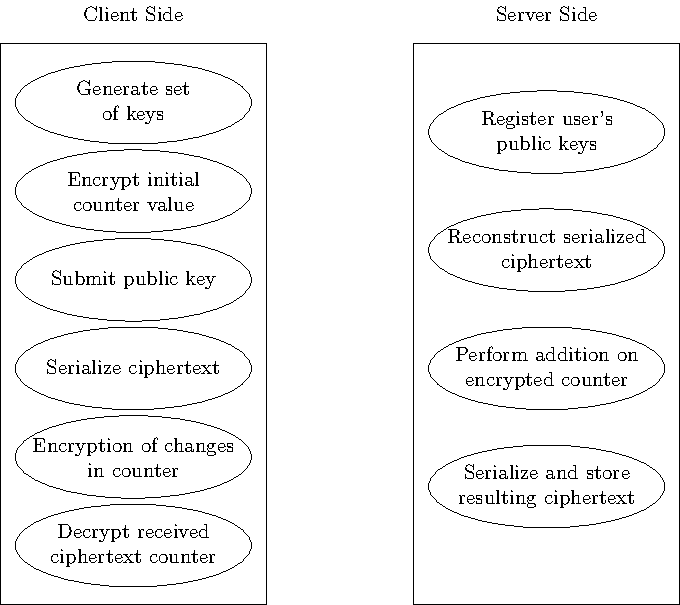
\includegraphics[scale=1]{img/architecture}
 \caption{Architecture breakdown into client and server.}
 \label{fig:clientserver}
\end{figure}

In order to understand how the workflow occurs inside of the client-server architecture, it is better to think of two possible clients: one that is located at the household, and another one that requests access to the counter data. The sensor system is the former one, whereas the user is the latter. Usually, the client that retrieves data from the sensor begins by generating a set of keys and registering it with the server, and then encrypting the value of the initial counter before sending it over. Whenever a change of the value is notified to the server, it performs the corresponding operations: addition if people go inside, or subtraction if people go outside the building. Finally, whenever the user wants to learn the value of the counter, it can request to download it from the server. It is also possible for the user to reset the value of the counter as he sees fit. This flow of operation is shown in Figure \ref{fig:seqdiag} as a sequence diagram.

\begin{figure}[H]
  \centering
  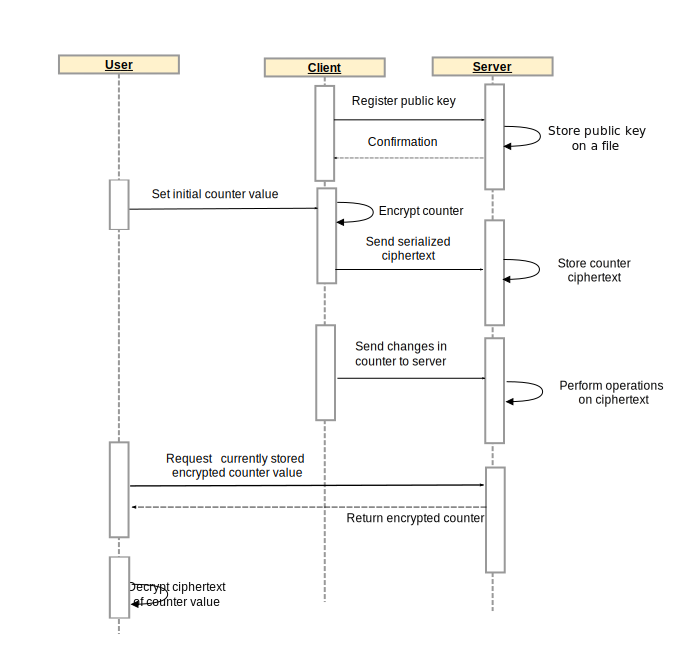
\includegraphics[width=\textwidth]{img/counter}
  \caption{Sequence diagram showing operation under normal conditions}
  \label{fig:seqdiag}
\end{figure}

\section{Discussion}

The aspect of user registration is not part of the planned implementation itself, but it is recommended to consider how to handle different users. There might many more than a couple of households that make use of such a counting service. This is why each resident would have to register his public key and go through some kind of authentication mechanism every time they restart or download the counter data. It is especially important to take the appropriate measures so that somebody else does not reset the counter value of a household that is not theirs, because it would be chaotic when the resident looks at the counter and finds a value that does not represent a truthful status.
To keep the registration under control, it might be ideal to keep a list of registered users either on a database or on a simple file for each household which would contain basic pieces of information such as an email address or username, along with the hash value of a password and the appropriate public key for the household that is being registered.

There were several problems at this stage that were directly related to the implementation. The transmission of serialized data between the client and server was especially problematic. The early attempts at sending serialized data to the server were not quite successful. Many different kind of errors were found, and the most common one was related to memory allocation. After going through several trial and error attempts, it was found that the errors started appearing as the message got larger. This seemed to be inevitable as the default settings of a TCP blocking socket were not adequate to send large pieces of data. 

After doing the right adjustments, the problem seemed to go away, except that \textit{the result was not quite as expected}. It was known inmediately that something was up with the received ciphertext, as it could not decrypt properly. It helped to look at the data that the server received, and it was quite evident that it was not complete. Indeed, only certain fragments of the ciphertext were received successfully, which led to an incorrect decryption. Several adjustments were made to the process of receiving data, so that a couple of control variables were used to keep in check how many bytes were being received. It was set so that it would only stop reading data from the client until all of the bytes had been read and assembled in a buffer. Both the functionalities of reading and writing the ciphertext on a socket were relatively more complicated considering that it was done without the support of a framework that specialized on it.

%[TALK ABOUT DECRYPTION]
%(1 month later)->I forgot what i was going to say about decryption anyways

In summary, a description of the case study was given, a solution based on homomorphic encryption was proposed to tackle the problem found in the case study, details of the HElib were discussed, and all of the relevant considerations pertaining to the implementation were explained. These considerations took on points such as the parameters and context, key generation and serialization, software architecture, transmission of serialized data, reconstruction of the ciphertext, and applying changes to the counter. Finally, all of these tasks were addressed when considering a client-server implementation.

\clearpage

%\include{caseStudy}
\chapter{Experiments and Results}
\label{results}

This section describes the design of the experiments related to the use of fully homomorphic encryption in HElib, as well as a summary of the results obtained. The objective of the experimental design was to test whether or not homomorphic encryption was practical enough to be applied in the cloud as a web application. The feasibility of application in the web depends heavily on the time required to perform homomorphic evaluations, which is affected by several factors. One of these main factors is the \emph{security parameter} $k$, which is a value closely related to the generation of public and private keys and how secure they are. The experimental design consists in changing the $k$ parameter to different values, as to see to what degree it has impact on the key generation, encryption, decryption and addition \emph{processing times}, as well as the \emph{size} of the resulting public key and ciphertext. Finally, the results obtained are presented and briefly discussed. 

\section{Setup}

The experiment is performed by running several iterations of the program that runs in the underlying client-server architecture, as to evaluate how the security parameter $k$ affects the time required for certain activities in the software, such as key generation, encryption, decryption, and homomorphic addition of ciphertext. Evidently, processing encrypted data homomorphically needs more computation than operating on the plaintext directly. The ratio between both computations is called the \emph{overhead}, and it is evaluated in terms of time. The security parameter $k$ is considered important because the value affects how secure the resulting keys and ciphertexts become, as well as the overhead of performing homomorphic evaluations. In the design document by Halevi and Shoup \cite{cryptoeprint:2014:106}, it does not specify to what degree changing the value of $k$ would make the cipher vulnerable to cryptanalysis or a brute-force attack; however, it does specify that the technique they propose uses a \emph{ciphertext packing} circuit that can be evaluated homomorphically in time $T \cdot $polylog($k$), which represents the overhead of the computation. Assuming the use of a circuit model of computation, the security parameter $k$ describes the width of the circuit being evaluated homomorphically.

To show how the $k$ security parameter affects the operation of the homomorphic encryption program, the experiment considers several arbitrarily chosen values, namely: 20, 40, 80, 100; where 80 is the default value found in the examples of the HElib. Each value is seen as a \emph{treatment} in the experimental design. For each treatment, the program is run through \textbf{20 iterations} of key generation, encryption, decryption and addition. 

In order to perform the necessary iterations, certain parts of the code from both the client and server sides were taken and adjusted, so that all the operations were performed on the same program. Consequently, overhead operation costs such as sending data between the client and server are not considered for this experiment.

When generating the public and private keys, all of the other parameters are kept \emph{intact}, so that it is only the $k$ value that gets changed. Consequently, the other mechanisms slightly vary because they make use of the previously generated public key.

It is important to consider that the experimentation was done on a notebook which had an AMD Elite A4-5150M processor. The processor is dual core and it runs at 2.7 GHz. Therefore, the results might differ depending on the processor used.% Implementation and experimentation of the client-server homomorphic counter solution were done on GNU Linux in the Xubuntu 14.04 distribution.

\section{Results}

The results are presented in Table \ref{tbl:results}, where the column represents the characteristic or attribute considered, such as the processing times and the size of the public key and ciphertext files measured in bytes. Consider that the values presented are the averages obtained from the set of iterations run.

\begin{table}[h]
  \caption{Experimental results}
  \label{tbl:results}
\begin{tabular}{lrrrrrr}
k   & Key Gen. & Key Size  & Encryption & Decryption & Addition & Ctext Size \\
40  & 13.130 s & 165.922 MB & 0.355 s    & 0.048 s    & 0.074 s  & 30.977 kB        \\
60  & 10.710 s & 91.635 MB  & 0.414 s    & 0.056 s    & 0.077 s  & 36.053 kB        \\
80  & 8.380 s  & 57.080 MB  & 0.642 s    & 0.057 s    & 0.082 s  & 37.745 kB        \\
100 & 9.529 s  & 35.453 MB  & 0.579 s    & 0.064 s    & 0.082 s  & 43.676 kB
\end{tabular}
\end{table}

In order to illustrate the differences observed, Figure \ref{fig:boxplot} depicts a box plot that shows the time required to generate the set of keys depending on the size of $k$. It was chosen not to plot the data pertaining to the rest of the attributes under experimentation, mostly because the differences observed were not significant.

\begin{figure}[h]
  \centerline{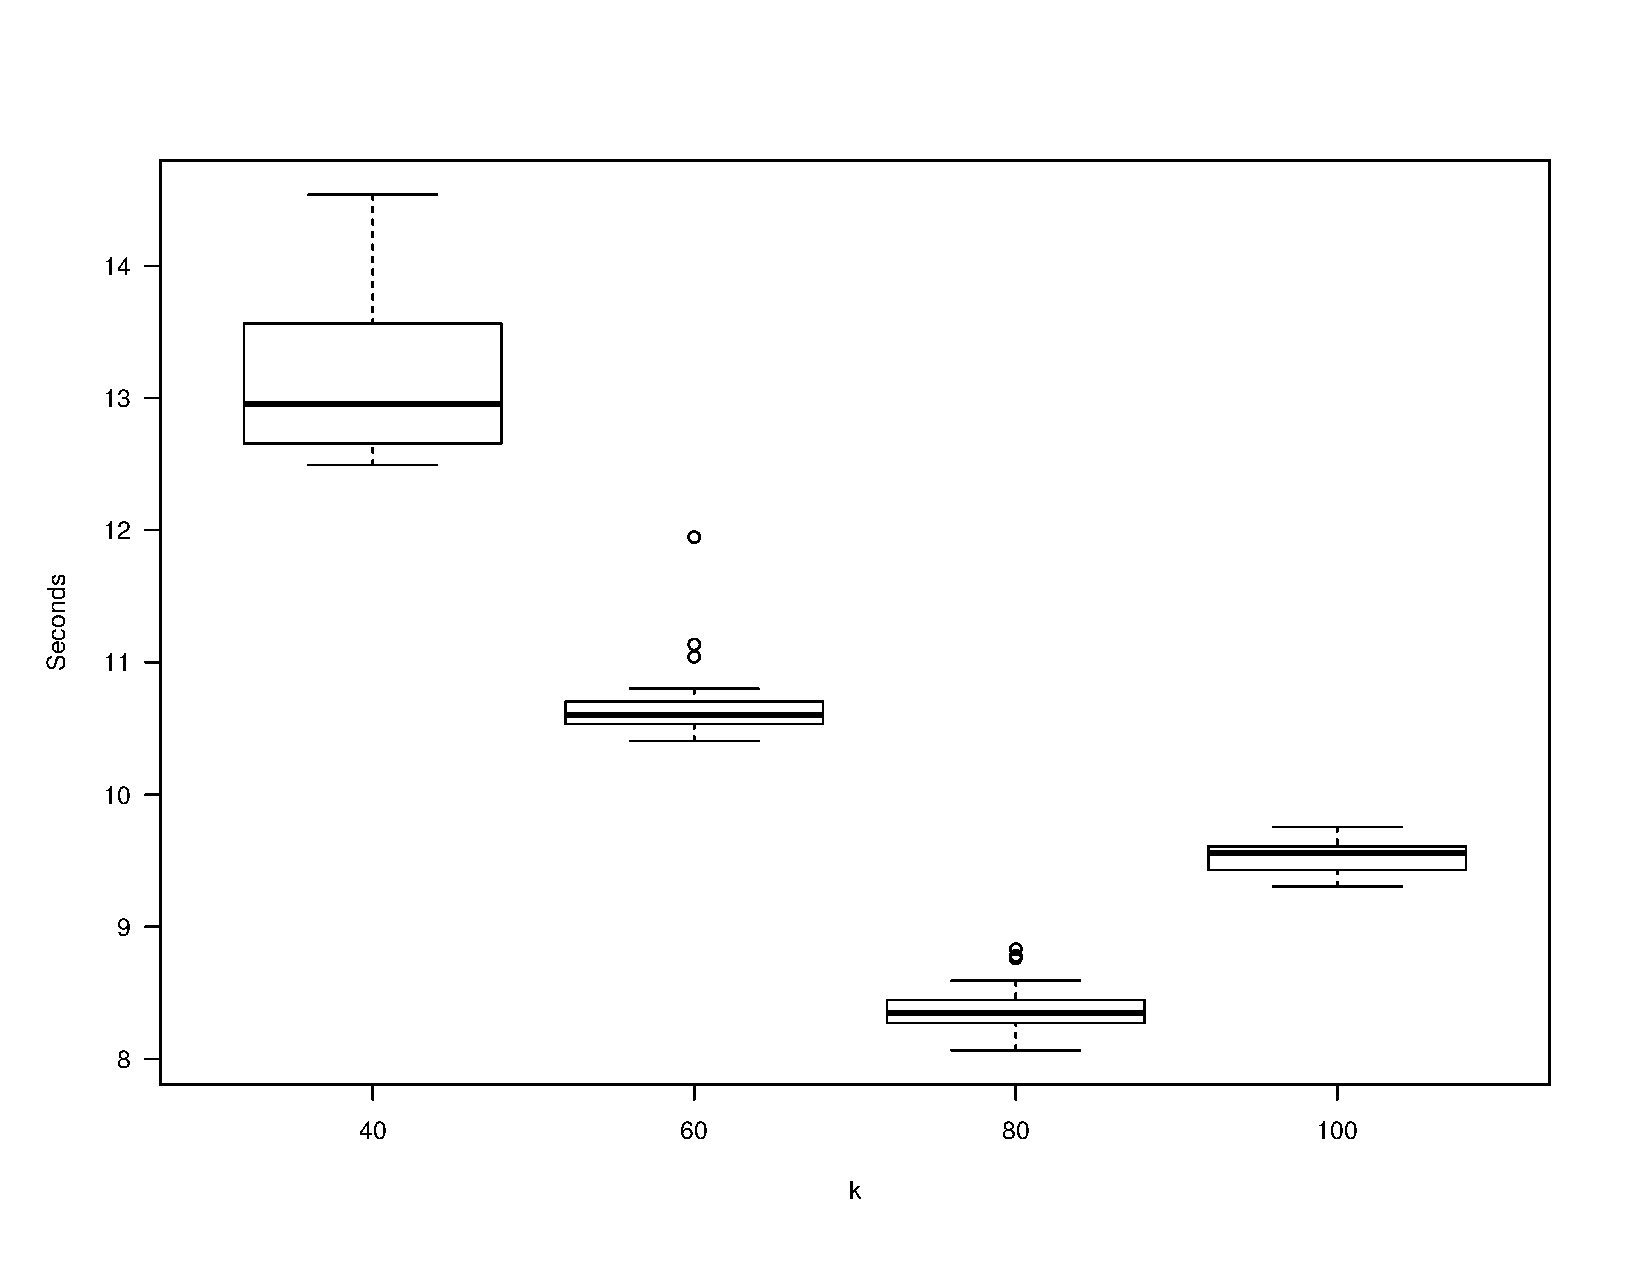
\includegraphics[height=7.5cm]{img/experimentplot}}
  \caption{Key generation time}
  \label{fig:boxplot}
\end{figure}


\section{Discussion}

The first characteristic that is being evaluated is the time needed to generate the set of public and private keys. Usually, the generation of keys is performed only once per user. Only if the private key were compromised, would the user create a new set of keys. Even though the highest average was 13 seconds for $k=40$, it is a relatively small amount of time. Directly linked to the generation of keys, the size of the key is considered relevant as well. Usually, the public key has to be shared with others, and in this particular case, the averages range between 165.92 MB for $k=40$  and 35.45 MB for $k=100$. The difference between both sizes is quite large, and even smallest key is significantly large by itself. Additionally, it is puzzling as to why the size of the public key is decreasing as the $k$ parameter gets larger. In cryptography, a larger $k$ usually implies a slowdown in the whole process, but in this case, it does quite the opposite, at least on the time needed for key generation.

%Preguntarte si los cambios son poco significativos

Regarding the encryption, decryption, and addition times, the average amount of time required is quite low, and it should not become a bottleneck even if many homomorphic evaluations are performed. Even though the encryption times are longer than the decryption times, none of them surpassed 1 second, which makes it quite acceptable in application. 

Perhaps the most important point to consider is the size of the generated ciphertexts. In the proposed architecture, a ciphertext is constantly sent to the server to perform operations and back to the client for decryption. According to the iterations run, the max average of the ciphertext size was found to be 43.67 kB for $k=100$, while smallest average was 30.99 kB for $k=40$. Looking at how the ciphertext sizes increases, it can be seen that it has a proportional relationship with the security parameter $k$. As $k$ gets larger, so does the size of the ciphertext. This would mean that higher security sacrifices storage, and consequently takes more time to transfer between the client and server.

Even assumming that a security parameter of $k=100$ is used, this shows that the size of the ciphertext is sufficiently small to be used in a web application hosted in the cloud. However, while the client-server architecture program was being developed, an average size of 74 MB per ciphertext was noted. At this time, it is not possible to recreate the scenario where ciphertexts of such a size were created, which leads to the impression that there is another factor not considered that accounts for the size of the ciphertext.

In conclusion, the aforementioned findings suggest that using HElib to apply homomorphic encryption in the cloud might indeed be feasible; however, as it has been noted, there are unknown circumstances that affect the size of the ciphertext. To the best of our knowledge, there is yet no way to predict the size of the ciphertext by using HElib. Therefore, if it is possible to keep the size of the ciphertext below 45kB, then it would certainly be feasible to take this solution to the cloud; otherwise, it would not be possible if each ciphertext had a size that exceeded several MB. Until these circumstances are made clear and evaluated properly, it is not possible at this time to show that using HElib to make use of homomorphic encryption in the cloud is indeed feasible. 

% Ver otra manera de poner la ultima oracion

\clearpage

%\include{existentes}

%\chapter{Soluci\'{o}n propuesta}
\label{propuesta}

rollo (estructura)

\section{Casos de uso}
\label{casosDeUso}

La figura \ref{casosDeUso} tiene, pues, casos de uso.


   {4:7} Beloved, let us love one another: for love is of God; and
every one that loveth is born of God, and knoweth God. {4:8} He that
loveth not knoweth not God; for God is love. {4:9} In this was
manifested the love of God toward us, because that God sent his only
begotten Son into the world, that we might live through him. {4:10}
Herein is love, not that we loved God, but that he loved us, and sent
his Son [to be] the propitiation for our sins. {4:11} Beloved, if God
so loved us, we ought also to love one another. {4:12} No man hath seen
God at any time. If we love one another, God dwelleth in us, and his
love is perfected in us. {4:13} Hereby know we that we dwell in him,
and he in us, because he hath given us of his Spirit. {4:14} And we
have seen and do testify that the Father sent the Son [to be] the
Saviour of the world. {4:15} Whosoever shall confess that Jesus is the
Son of God, God dwelleth in him, and he in God. {4:16} And we have
known and believed the love that God hath to us. God is love; and he
that dwelleth in love dwelleth in God, and God in him. {4:17} Herein is
our love made perfect, that we may have boldness in the day of
judgment: because as he is, so are we in this world. {4:18} There is no
fear in love; but perfect love casteth out fear: because fear hath
torment. He that feareth is not made perfect in love. {4:19} We love
him, because he first loved us. {4:20} If a man say, I love God, and
hateth his brother, he is a liar: for he that loveth not his brother
whom he hath seen, how can he love God whom he hath not seen? {4:21}
And this commandment have we from him, That he who loveth God love his
brother also.

\begin{figure}[t]
\begin{center}
\begin{tikzpicture} 

\umlusecase[x=4, y=0]{Registro} 
\umlusecase[x=4, y=-2]{Seleccion} 

\umlactor{Alumno} 
\umlactor[y=-3]{Responsable del departamento escolar} 
\umlactor[x=9, y=-1]{Administrador del sistema}

\end{tikzpicture}
\end{center}
\caption{Casos de uso}
\label{casosDeUso}
\end{figure}


The First Epistle General of John

   {1:1} That which was from the beginning, which we have heard, which
we have seen with our eyes, which we have looked upon, and our hands
have handled, of the Word of life; {1:2} (For the life was manifested,
and we have seen [it,] and bear witness, and shew unto you that eternal
life, which was with the Father, and was manifested unto us;) {1:3}
That which we have seen and heard declare we unto you, that ye also may
have fellowship with us: and truly our fellowship [is] with the Father,
and with his Son Jesus Christ. {1:4} And these things write we unto
you, that your joy may be full.

   {1:5} This then is the message which we have heard of him, and
declare unto you, that God is light, and in him is no darkness at all.
{1:6} If we say that we have fellowship with him, and walk in darkness,
we lie, and do not the truth: {1:7} But if we walk in the light, as he
is in the light, we have fellowship one with another, and the blood of
Jesus Christ his Son cleanseth us from all sin. {1:8} If we say that we
have no sin, we deceive ourselves, and the truth is not in us. {1:9} If
we confess our sins, he is faithful and just to forgive us [our] sins,
and to cleanse us from all unrighteousness. {1:10} If we say that we
have not sinned, we make him a liar, and his word is not in us.

   {2:1} My little children, these things write I unto you, that ye sin
not. And if any man sin, we have an advocate with the Father, Jesus
Christ the righteous: {2:2} And he is the propitiation for our sins:
and not for ours only, but also for [the sins of] the whole world.
{2:3} And hereby we do know that we know him, if we keep his
commandments. {2:4} He that saith, I know him, and keepeth not his
commandments, is a liar, and the truth is not in him. {2:5} But whoso
keepeth his word, in him verily is the love of God perfected: hereby
know we that we are in him. {2:6} He that saith he abideth in him ought
himself also so to walk, even as he walked.

   {2:7} Brethren, I write no new commandment unto you, but an old
commandment which ye had from the beginning. The old commandment is the
word which ye have heard from the beginning. {2:8} Again, a new
commandment I write unto you, which thing is true in him and in you:
because the darkness is past, and the true light now shineth. {2:9} He
that saith he is in the light, and hateth his brother, is in darkness
even until now. {2:10} He that loveth his brother abideth in the light,
and there is none occasion of stumbling in him. {2:11} But he that
hateth his brother is in darkness, and walketh in darkness, and knoweth
not whither he goeth, because that darkness hath blinded his eyes.
{2:12} I write unto you, little children, because your sins are
forgiven you for his name's sake. {2:13} I write unto you, fathers,
because ye have known him [that is] from the beginning. I write unto
you, young men, because ye have overcome the wicked one. I write unto
you, little children, because ye have known the Father. {2:14} I have
written unto you, fathers, because ye have known him [that is] from the
beginning. I have written unto you, young men, because ye are strong,
and the word of God abideth in you, and ye have overcome the wicked
one. {2:15} Love not the world, neither the things [that are] in the
world. If any man love the world, the love of the Father is not in him.
{2:16} For all that [is] in the world, the lust of the flesh, and the
lust of the eyes, and the pride of life, is not of the Father, but is
of the world. {2:17} And the world passeth away, and the lust thereof:
but he that doeth the will of God abideth for ever.

   {2:18} Little children, it is the last time: and as ye have heard
that antichrist shall come, even now are there many antichrists;
whereby we know that it is the last time. {2:19} They went out from us,
but they were not of us; for if they had been of us, they would [no
doubt] have continued with us: but [they went out,] that they might be
made manifest that they were not all of us. {2:20} But ye have an
unction from the Holy One, and ye know all things. {2:21} I have not
written unto you because ye know not the truth, but because ye know it,
and that no lie is of the truth. {2:22} Who is a liar but he that
denieth that Jesus is the Christ? He is antichrist, that denieth the
Father and the Son. {2:23} Whosoever denieth the Son, the same hath not
the Father: [(but) he that acknowledgeth the Son hath the Father also.
]{2:24} Let that therefore abide in you, which ye have heard from the
beginning. If that which ye have heard from the beginning shall remain
in you, ye also shall continue in the Son, and in the Father. {2:25}
And this is the promise that he hath promised us, [even] eternal life.
{2:26} These [things] have I written unto you concerning them that
seduce you. {2:27} But the anointing which ye have received of him
abideth in you, and ye need not that any man teach you: but as the same
anointing teacheth you of all things, and is truth, and is no lie, and
even as it hath taught you, ye shall abide in him. {2:28} And now,
little children, abide in him; that, when he shall appear, we may have
confidence, and not be ashamed before him at his coming. {2:29} If ye
know that he is righteous, ye know that every one that doeth
righteousness is born of him.

   {3:1} Behold, what manner of love the Father hath bestowed upon us,
that we should be called the sons of God: therefore the world knoweth
us not, because it knew him not. {3:2} Beloved, now are we the sons of
God, and it doth not yet appear what we shall be: but we know that,
when he shall appear, we shall be like him; for we shall see him as he
is. {3:3} And every man that hath this hope in him purifieth himself,
even as he is pure. {3:4} Whosoever committeth sin transgresseth also
the law: for sin is the transgression of the law. {3:5} And ye know
that he was manifested to take away our sins; and in him is no sin.
{3:6} Whosoever abideth in him sinneth not: whosoever sinneth hath not
seen him, neither known him. {3:7} Little children, let no man deceive
you: he that doeth righteousness is righteous, even as he is righteous.
{3:8} He that committeth sin is of the devil; for the devil sinneth
from the beginning. For this purpose the Son of God was manifested,
that he might destroy the works of the devil. {3:9} Whosoever is born
of God doth not commit sin; for his seed remaineth in him: and he
cannot sin, because he is born of God. {3:10} In this the children of
God are manifest, and the children of the devil: whosoever doeth not
righteousness is not of God, neither he that loveth not his brother.
{3:11} For this is the message that ye heard from the beginning, that
we should love one another. {3:12} Not as Cain, [who] was of that
wicked one, and slew his brother. And wherefore slew he him? Because
his own works were evil, and his brother's righteous.

   {3:13} Marvel not, my brethren, if the world hate you. {3:14} We
know that we have passed from death unto life, because we love the
brethren. He that loveth not [his] brother abideth in death. {3:15}
Whosoever hateth his brother is a murderer: and ye know that no
murderer hath eternal life abiding in him. {3:16} Hereby perceive we
the love [of God,] because he laid down his life for us: and we ought
to lay down [our] lives for the brethren. {3:17} But whoso hath this
world's good, and seeth his brother have need, and shutteth up his
bowels [of compassion] from him, how dwelleth the love of God in him?
{3:18} My little children, let us not love in word, neither in tongue;
but in deed and in truth. {3:19} And hereby we know that we are of the
truth, and shall assure our hearts before him. {3:20} For if our heart
condemn us, God is greater than our heart, and knoweth all things.
{3:21} Beloved, if our heart condemn us not, [then] have we confidence
toward God. {3:22} And whatsoever we ask, we receive of him, because we
keep his commandments, and do those things that are pleasing in his
sight. {3:23} And this is his commandment, That we should believe on
the name of his Son Jesus Christ, and love one another, as he gave us
commandment. {3:24} And he that keepeth his commandments dwelleth in
him, and he in him. And hereby we know that he abideth in us, by the
Spirit which he hath given us.

   {4:1} Beloved, believe not every spirit, but try the spirits whether
they are of God: because many false prophets are gone out into the
world. {4:2} Hereby know ye the Spirit of God: Every spirit that
confesseth that Jesus Christ is come in the flesh is of God: {4:3} And
every spirit that confesseth not that Jesus Christ is come in the flesh
is not of God: and this is that [spirit] of antichrist, whereof ye have
heard that it should come; and even now already is it in the world.
{4:4} Ye are of God, little children, and have overcome them: because
greater is he that is in you, than he that is in the world. {4:5} They
are of the world: therefore speak they of the world, and the world
heareth them. {4:6} We are of God: he that knoweth God heareth us; he
that is not of God heareth not us. Hereby know we the spirit of truth,
and the spirit of error.

   {5:1} Whosoever believeth that Jesus is the Christ is born of God:
and every one that loveth him that begat loveth him also that is
begotten of him. {5:2} By this we know that we love the children of
God, when we love God, and keep his commandments. {5:3} For this is the
love of God, that we keep his commandments: and his commandments are
not grievous. {5:4} For whatsoever is born of God overcometh the world:
and this is the victory that overcometh the world, [even] our faith.
{5:5} Who is he that overcometh the world, but he that believeth that
Jesus is the Son of God? {5:6} This is he that came by water and blood,
[even] Jesus Christ; not by water only, but by water and blood. And it
is the Spirit that beareth witness, because the Spirit is truth. {5:7}
For there are three that bear record in heaven, the Father, the Word,
and the Holy Ghost: and these three are one. {5:8} And there are three
that bear witness in earth, the spirit, and the water, and the blood:
and these three agree in one. {5:9} If we receive the witness of men,
the witness of God is greater: for this is the witness of God which he
hath testified of his Son. {5:10} He that believeth on the Son of God
hath the witness in himself: he that believeth not God hath made him a
liar; because he believeth not the record that God gave of his Son.
{5:11} And this is the record, that God hath given to us eternal life,
and this life is in his Son. {5:12} He that hath the Son hath life;
[and] he that hath not the Son of God hath not life. {5:13} These
things have I written unto you that believe on the name of the Son of
God; that ye may know that ye have eternal life, and that ye may
believe on the name of the Son of God. {5:14} And this is the
confidence that we have in him, that, if we ask any thing according to
his will, he heareth us: {5:15} And if we know that he hear us,
whatsoever we ask, we know that we have the petitions that we desired
of him. {5:16} If any man see his brother sin a sin [which is] not unto
death, he shall ask, and he shall give him life for them that sin not
unto death. There is a sin unto death: I do not say that he shall pray
for it. {5:17} All unrighteousness is sin: and there is a sin not unto
death. {5:18} We know that whosoever is born of God sinneth not; but he
that is begotten of God keepeth himself, and that wicked one toucheth
him not. {5:19} And we know that we are of God, and the whole world
lieth in wickedness. {5:20} [And] we know that the Son of God is come,
and hath given us an understanding, that we may know him that is true,
and we are in him that is true, [even] in his Son Jesus Christ. This is
the true God, and eternal life. {5:21} Little children, keep yourselves
from idols. Amen.






\clearpage

%\include{evaluacion}
\chapter{Conclusions and Future Work}
\label{conclusions}

We showed the design and implementation of a client-server architecture based software that employs homomorphic encryption in order to perform computations on encrypted data. The software relies on the HElib library to enable the necessary homomorphic evaluations. The work focused on the confidentiality of a household counting system as case study. 

A set of public and private keys were created by the client using certain parameters, and the former key was sent to the server. The server registered the public key for future use. An initial value representing the number of people inside the household was chosen and encrypted using the client's public key. The ciphertext resulting from the encryption of the counter value was serialized into a container. Once the communication between server and client was established, the serialized ciphertext was sent to the server using sockets on the TCP. Whenever a change in the amount of individuals inside the household was recorded, the server was promptly informed of it. The server reconstructed the ciphertext representing the initial value using the appropriate public key, and performed an addition between the original value and its respective change. Then, the client requested to see the modified counter value, to which the server responded by sending the modified ciphertext. Finally, the client decrypted the received ciphertext by using its private key, and confirmed the current counter value. 

In essense, a client-server archictecture was established and it made use of homomorphic encryption successfully. It was found that the factors that pose a challenge to deem applications of homomorphic encryption as inefficient were mainly: key generation time, key size, ciphertext size, and encryption and decryption times. Moreover, the client-server software implementation showed as simple as possible how HElib can be used to fulfill the necessary use cases. 

In order to confirm the relevant factors pertaining to the feasibility of an implementation in the cloud, data regarding the execution times and size of the key and ciphertext were collected.It was chosen to experiment on the value of the $k$ security parameter, since it was apparent that it had the most impact on the operations performed by the library. 

The results showed that key generation took the most amount of time, ranging between 9 and 13 seconds. The size of the public key ranged between 35 and 165 megabytes. Despite the long time and large size, these were not considered to be obstacles to the feasibility of the system. This is because key generation and registration of the public key is done only at the beginning of the process and is not required to do it again at a later time.

\section{Final Remarks}

It was noted during the development phase that the ciphertext often had a filesize of around 74 megabytes, and it was surprising to see that this value got reduced to less than 50 kilobytes during the experimentation phase. It is not clear which factors influenced the drastic change during these phases, and it made it difficult to decide whether implementing this as a service in the cloud would be feasible or not. In the case that the ciphertext size is indeed too large, the design of the system could be tweaked so that only the initial value of the counter is encrypted, so that the change values are sent to the server as plaintext. Evidently, this would diminish the overall security of the system, since it would not be impossible to predict the current value of the counter by observing the changes. 

\section{Contributions}

The main contribution of this work is the design and implementation of a client-server architecture based software that employs homomorphic encryption. The proposed system addresses the processes regarding key generation, data encryption, client-server communication, addition on encrypted data, and decryption. It is relevant to note that this system relies on the homomorphic encryption functionalities provided by the HElib library. The contribution itself is related to how the library is being used to implement a system in a client-server model.

Regarding the proposed system, the following points are important to mention:

\begin{itemize}
\item The overall process was designed around a case study that had the goal of counting the number of people inside a household while maintaining its confidentiality. Neither the server nor other other authorized parties are able to learn of the value of the counter, as they do not have the private key that is required for decryption.
\item As the counter data was encrypted, further changes to it were performed by using homomorphic addition. 
\item Serialization was used in order to send the public key and ciphertext with the server.
\item As proof of concept, socket communication that relied on TCP was used between client and server to transmit the required data.
\end{itemize} 

\section{Future Work}
At a first glance, the results obtained from the experimentation were satisfactory; however, some doubts were raised upon noticing that there was a great variation between the development and experimentation phases of the ciphertext size. More experimentation is recommended to fully ascertain what other factors have an impact in the size of the ciphertext. As future work, the following points are noted:

\begin{itemize}
\item Design and implement the appropriate mechanisms for key management, including key registration.
\item Design a database scheme to keep control of the ciphertexts stored in the server, while associating each of them with its respective public key.
\item Look into the possibility of implementing the client-architecture system as a Software-as-a-Service model.
\item Provide a secure communication channel between the client and server, relying on the SSL protocol.
\item Experiment on the number of homomorphic operations correctly evaluated before the accumulated noise causes an incorrect decryption.
\item Implement solution over the HTTP protocol, as to allow use via web browsers.
\end{itemize}

\clearpage


%\bibliographystyle{plain}
\bibliographystyle{estiloDeBibliografiaJorge}
\bibliography{bibliografia}

%\appendix
%\include{Apendice}

\printindex{}
\backmatter
\pagestyle{main}
%%Autobiografia

\chapter*{Ficha autobiogr�fica}
\chaptermark{Ficha autobiogr�fica}

\begin{center}
\autor

Candidato para el grado de \grado.

\uanl

\fime\bigskip

Tesis:
	
\begin{tabular}{p{11cm}}
	\centering
	\scshape{\large{\titulo}}
\end{tabular}
\end{center}

\bigskip

Nac\'{\i} el \ldots

\label{lastpage}


\end{document}
